\ExerciseSection

\begin{enumerate}
\def\labelenumi{\arabic{enumi})}
\tightlist
\item
  \begin{enumerate}
  \def\labelenumii{\alph{enumii})}
  \tightlist
  \item
    If A is a subset of a topological space X, show that the following statements are equivalent: \(\alpha\) the frontier of A is nowhere dense; \(\beta\) A is the union of an open set and a nowhere dense set; \(\gamma\) A is the difference between a closed set and a nowhere dense set.
  \end{enumerate}
\end{enumerate}

\begin{enumerate}
\def\labelenumi{\alph{enumi})}
\setcounter{enumi}{1}
\tightlist
\item
  Show that if a subset A of X is such that, for each point \(x \in A\) , there is a neighbourhood V of x in X such that \(V \cap A\) is nowhere dense in X, then A is nowhere dense in X.
\end{enumerate}

\begin{enumerate}
\def\labelenumi{\arabic{enumi})}
\setcounter{enumi}{1}
\tightlist
\item
  A subset \(\mathbf{A}\) of a topological space \(\mathbf{X}\) is said to be a thin set if, for each perfect set \(\mathbf{P} \subset \mathbf{X}\) , \(\mathbf{P} \cap \mathbf{A}\) is nowhere dense in \(\mathbf{P}\) .
\end{enumerate}

\begin{enumerate}
\def\labelenumi{\alph{enumi})}
\item
  Every finite union of thin sets is thin.
\item
  The frontier of a thin set is nowhere dense.
\item
  There is a largest perfect set in \(\mathbf{X}\) whose complement is thin.
\end{enumerate}

\begin{enumerate}
\def\labelenumi{\arabic{enumi})}
\setcounter{enumi}{2}
\tightlist
\item
  Let A be a subset of a topological space X, and let D(A) denote the set of all \(x \in X\) such that, for each neighbourhood V of x, the set \(V \cap A\) is not meagre. D(A) is contained in \(\overline{A}\) .
\end{enumerate}

\begin{enumerate}
\def\labelenumi{\alph{enumi})}
\tightlist
\item
  If \(\mathbf{B}\) is a subset of \(\mathbf{X}\) such that \(\mathbf{D}(\mathbf{B}) = \varnothing\) , then
\end{enumerate}

\[
\mathbf {D} (\mathbf {A} \cup \mathbf {B}) = \mathbf {D} (\mathbf {A})
\]

for every subset A of X.

\begin{enumerate}
\def\labelenumi{\alph{enumi})}
\setcounter{enumi}{1}
\item
  D(A) = ∅ if and only if A is meagre. {[}Begin by showing that if (U\_t) is a family of pairwise disjoint open subsets of X and if, for each t, V\_t is a nowhere dense set (relative to X) contained in U\_t, then ∪ V\_t is nowhere dense. Then consider a maximal set M of open subsets of X, each pair of which are disjoint, and such that A ∪ U is meagre for each U ∈ M; the existence of such a maximal set is established by Zorn's lemma. Show that if D(A) = ∅, then A ∩ C W is nowhere dense, where W is the union of the sets of M, and hence show that A is meagre.{]}
\item
  Show that \(\mathbf{D}(\mathbf{A})\) is closed and that \(\mathbf{A} \cap \mathbf{CD}(\mathbf{A})\) is meagre for all \(A \subset X\) {[}show, with the help of b), that \(\mathbf{A} \cap \mathbf{CD}(\mathbf{A})\) is meagre relative to the open subspace \(\mathbf{CD}(\mathbf{A})\) {]}.
\end{enumerate}

\(d\) ) Show that \(\mathbf{D}(\mathbf{A})\) is equal to the closure of its interior. {[}If \(\mathbf{D}'(\mathbf{A})\) is the closure of the interior of \(\mathbf{D}(\mathbf{A})\) , show that \(\mathbf{A} \cap \mathbb{C}\mathbf{D}'(\mathbf{A})\) is meagre, by observing that this set is the union of

\[
\mathbf {A} \cap \mathbb {C D} (\mathbf {A}) \quad \text { and } \quad \mathbf {A} \cap \mathbf {D} (\mathbf {A}) \cap \mathbb {C D} ^ {\prime} (\mathbf {A}). ]
\]

\begin{enumerate}
\def\labelenumi{\arabic{enumi})}
\setcounter{enumi}{3}
\tightlist
\item
  Let \(\mathbf{X}\) and \(\mathbf{Y}\) be two topological spaces and let \(\mathbf{A}\) (resp. B) be a subset of \(\mathbf{X}\) (resp. Y).
\end{enumerate}

\begin{enumerate}
\def\labelenumi{\alph{enumi})}
\item
  \(\mathbf{A} \times \mathbf{B}\) is nowhere dense (resp. perfect) in \(\mathbf{X} \times \mathbf{Y}\) if and only if one of the two sets \(\mathbf{A}, \mathbf{B}\) is nowhere dense (resp. \(\mathbf{A}\) and \(\mathbf{B}\) are closed and one of them is perfect).
\item
  \(\mathbf{A} \times \mathbf{B}\) is thin in \(\mathbf{X} \times \mathbf{Y}\) if and only if \(\mathbf{A}\) and \(\mathbf{B}\) are both thin sets.
\end{enumerate}

\begin{enumerate}
\def\labelenumi{\arabic{enumi})}
\setcounter{enumi}{4}
\tightlist
\item
  \begin{enumerate}
  \def\labelenumii{\alph{enumii})}
  \tightlist
  \item
    Let X and Y be two topological spaces and let A be a nowhere dense subset of \(X \times Y\) . If the topology of Y has a countable base, show that the set of all \(x \in X\) such that the section \(\mathbf{A} \cap (\{x\} \times \mathbf{Y})\) of A at x is not nowhere dense relative to \(\{x\} \times Y\) is a meagre set in X (if U is any non-empty open set in Y, show that the set of all \(x \in X\) such that \(\{x\} \times U\) is contained in the closure of the section of A at x is a nowhere dense set in X).
  \end{enumerate}
\end{enumerate}

\begin{enumerate}
\def\labelenumi{\alph{enumi})}
\setcounter{enumi}{1}
\item
  Show by an example that the result of a) can be false if the topology of Y does not have a countable base (take X to be a Hausdorff space with no isolated points and Y to be the set X with the discrete topology; and take A to be the diagonal of \(X \times Y\) ).
\item
  If B, C are subsets of X, Y respectively and if one of B, C is meagre (in X, Y respectively), then \(B \times C\) is meagre in \(X \times Y\) . Conversely, if \(B \times C\) is meagre in \(X \times Y\) and if the topology of either X or Y has a countable base, then one of the sets B, C is meagre.
\item
  Deduce from c) that if the topology of one of the spaces X, Y has a countable base, then \(\mathrm{D}(\mathbf{B} \times \mathbf{C}) = \mathrm{D}(\mathbf{B}) \times \mathrm{D}(\mathbf{C})\) in the notation of Exercise 3.
\end{enumerate}

\begin{enumerate}
\def\labelenumi{\arabic{enumi})}
\setcounter{enumi}{5}
\tightlist
\item
  A set A in a topological space X is said to be almost open if there is an open set U in X such that both \(U \cap C A\) and \(A \cap C U\) are meagre sets.
\end{enumerate}

\begin{enumerate}
\def\labelenumi{\alph{enumi})}
\item
  The complement of an almost open set is almost open.
\item
  Any countable union of almost open sets is almost open.
\item
  Show that the following statements are equivalent: \(\alpha\) ) A is almost open; \(\beta\) ) there is a meagre subset M of X such that A∩CM is both open and closed in the subspace X---M; \(\gamma\) ) there is a set G⊂A which is a countable intersection of open sets in X, such that A---G is meagre in X; \(\delta\) ) there is a set F⊃A which is a countable union of closed sets in X, such that F---A is meagre in X; \(\zeta\) ) the set D(A)∩D(X---A) (Exercise 3) is nowhere dense in X; \(\theta\) ) the set D(A)∩CA is meagre in X. {[}Use Exercises 3a) and 3b) to show that \(\alpha)\Longrightarrow\zeta)\Longrightarrow\theta)\Longrightarrow\alpha\).{]} d) Let X, Y be two topological spaces and suppose that the topology of either X or Y has a countable base. Then a subset of X × Y of the form \(\mathbf{A} \times \mathbf{B}\) is almost open if and only if either both \(\mathbf{A}\) and \(\mathbf{B}\) are almost open or one of them is meagre {[}use \(\zeta\) ) of \(c\) {]}.
\end{enumerate}

\begin{enumerate}
\def\labelenumi{\arabic{enumi})}
\setcounter{enumi}{6}
\tightlist
\item
  A topological space X is said to be non-meagre if it is not meagre relative to itself.
\end{enumerate}

\begin{enumerate}
\def\labelenumi{\alph{enumi})}
\item
  X is non-meagre if and only if every countable family of dense open sets in X has a non-empty intersection.
\item
  In a non-meagre space, the complement of every meagre set is a non-meagre subspace.
\end{enumerate}

\begin{enumerate}
\def\labelenumi{\arabic{enumi})}
\setcounter{enumi}{7}
\item
  Let X be a topological space in which there is a non-empty open subset A which is a non-meagre subspace. Show that X is non-meagre and that A is not a meagre set relative to X.
\item
  Let X be the subspace of \(R^{2}\) which is the union of \(Q^{2}\) and the line y = 0. Show that X is meagre relative to itself. Deduce that a topological space can have non-meagre subspaces without being non-meagre itself.
\item
  Show that every completely regular pseudo-compact space (§ 1, Exercise 21) is a Baire space (argue as in Theorem 1).
\item
  If X is a Baire space with no isolated points, show that every point of X is a point of condensation of X (Chapter I, § 9, Exercise 17).
\end{enumerate}

¶ 12) A topological space X is said to be totally non-meagre if every non-empty closed subspace of X is non-meagre. A locally compact space is totally non-meagre, and so is a complete metric space.

\begin{enumerate}
\def\labelenumi{\alph{enumi})}
\item
  Show that a totally non-meagre regular space is a Baire space.
\item
  In an accessible totally non-meagre space, a non-empty countable closed set is thin (Exercise 2) and hence has at least one isolated point.
\item
  In a totally non-meagre space X, every subspace A which is the intersection of a countable intersection of open sets in X is totally non-meagre (if F is a subset of A which is closed in A, let \(\overline{F}\) be the closure of F in X, and show that \(\overline{F} \cap C F\) is meagre relative to \(\overline{F}\) ).
\item
  If every point of a topological space X has a neighbourhood which is a totally non-meagre subspace, then X is totally non-meagre.
\end{enumerate}

¶ 13) Let X be a totally non-meagre space which is connected and locally connected. Show that X cannot be the union of an infinite sequence (F \(_{n}\) ) of non-empty mutually disjoint closed sets. (Let H be the union of the frontiers H \(_{n}\) of the F \(_{n}\) in X; show that H is closed in X and that each set H \(_{n}\) is nowhere dense in H; to establish the latter point, consider a fundamental system of connected neighbourhoods of a point of \(\mathbf{H}_n\) , and argue by contradiction, using Chapter I, § 11, Proposition 3.)

\begin{enumerate}
\def\labelenumi{\arabic{enumi})}
\setcounter{enumi}{13}
\tightlist
\item
  Let X be the subspace of \(R^{2}\) consisting of the points \((r,0)\) , where r runs through the set Q of rational numbers, and the points \((k/n,1/n)\) , where n runs through the set of integers \(\geqslant 1\) and k runs through the set of all rational integers. Show that X is a Baire space but is not totally non-meagre.
\end{enumerate}

¶ 15) Let X be the subset of the plane \(\mathbf{R}^2\) consisting of the line \(\mathrm{D} = \{0\} \times \mathbf{R}\) and the points \((1/n, k/n^2)\) , where \(n\) runs through the set of integers \(>0\) and \(k\) runs through the set of all rational integers. a) For each point \((0, y)\) of D and each integer \(n > 0\) , let \(\mathrm{T}_n(y)\) be the set of points \((u, v) \in \mathbf{X}\) such that \(u \leqslant 1/n\) and \(|v - y| \leqslant u\) . Show that if we take as a fundamental system of neighbourhoods of each point \((0, y)\) the set of sets \(\mathrm{T}_n(y)\) , and as a fundamental system of neighbourhoods of each other point of X the set consisting of this point alone, then we have defined a topology \(\mathcal{G}\) on X, which is finer than the topology induced by that of \(\mathbf{R}^2\) , and with respect to which X is locally compact. b) Show that X is the union of a countable family of metrizable closed subspaces and that every point of X has a metrizable compact neighbourhood, but that X is not normal. {[}Let A be the set of all points \((0, y)\) where \(y\) is rational, and let \(\mathbf{B} = \mathbf{D} - \mathbf{A}\) ; show that every neighbourhood U of A in X meets every neighbourhood V of B in X; for this, consider for each \(n\) the set \(\mathbf{B}_n\) of points \(y \in \mathbf{B}\) such that \(\mathrm{T}_n(y) \subset \mathbf{V}\) , and note that the set B is not meagre in R.{]}

¶ 16) Let \(\mathbf{R}_{-}\) denote the topological space obtained by endowing the linearly ordered set \(\mathbf{R}\) of real numbers with the topology \(\mathcal{G}_{-}(\mathbf{R})\) (Chapter I, § 2, Exercise 5).

\begin{enumerate}
\def\labelenumi{\alph{enumi})}
\item
  Show that every open set in \(\mathbf{R}_{-}\) is the union of a countable family of mutually disjoint intervals which are either open or half-open on the left. Deduce that \(\mathbf{R}_{-}\) is perfectly normal (§ 4, Exercise 8) and totally non-meagre (Exercise 12).
\item
  Show that the space \(\mathbf{R}_{-} \times \mathbf{R}_{-}\) is not normal, and hence that \(\mathbf{R}_{-}\) is not metrizable, although \(\mathbf{R}_{-}\) contains a countable dense subset. (Considering the set of points \((x, y)\) in \(\mathbf{R}_{-} \times \mathbf{R}_{-}\) such that \(x + y = 1\) , show that \(\mathbf{R}_{-} \times \mathbf{R}_{-}\) has a closed subspace which is homeomorphic to the space \(\mathbf{X}\) defined in Exercise 15.)
\item
  Show that \(\mathbf{R}_{-}\) is a Lindelöf space (Chapter I, § 9, Exercise 15) and therefore is paracompact (§ 4, Exercise 23). (For each \(x \in \mathbf{R}_{-}\) , let \(\mathbf{U}_x\) be a semi-open interval {]} \(y(x)\) , \(x]\) with \(x\) as right-hand end-point. Show that the set of \(z \in \mathbf{R}_{-}\) which do not belong to any open interval {]} \(y(x)\) , \(x[\) is countable; use Chapter IV, § 2, Exercise 1.)
\item
  Show that every compact subset of \(R_{-}\) is countable {[}if A is a compact set in \(R_{-}\) , the topologies induced on A by \(\mathcal{G}_{-}(\mathbf{R})\) and \(\mathcal{G}_{0}(\mathbf{R})\) are identical; deduce that every point of A is the left-hand end-point of an interval contiguous to A{]}.
\end{enumerate}

\begin{enumerate}
\def\labelenumi{\arabic{enumi})}
\setcounter{enumi}{16}
\tightlist
\item
  \begin{enumerate}
  \def\labelenumii{\alph{enumii})}
  \tightlist
  \item
    Show that every product \(\mathbf{X} = \prod_{i\in \mathbf{I}}\mathbf{X}_i\) of complete metric spaces is a Baire space. {[}Argue as in the proof of Theorem 1, taking \(\mathbf{G}_n\) to be an elementary set (Chapter I, § 4, no. 1) all of whose projections are either the whole space or have a diameter \(\leqslant 1 / n\) ; then note that there is a countable subset J of I such that each \(\mathbf{G}_n\) is of the form \(\mathbf{H}_n\times \prod_{i\notin \mathbf{J}}\mathbf{X}_i\) , where \(\mathbf{H}_n\subset \prod_{i\in \mathbf{J}}\mathbf{X}_i.\) {]}
  \end{enumerate}
\end{enumerate}

\begin{enumerate}
\def\labelenumi{\alph{enumi})}
\setcounter{enumi}{1}
\tightlist
\item
  Show by an example that if I is uncountable then X need not be totally non-meagre (Exercise 12). {[}Use Exercises 1 and 23 b) of § 2.{]}
\end{enumerate}

¶ 18) a) Show that in a complete metric space, every perfect set contains a subset homeomorphic to Cantor's triadic set (Chapter IV, § 2, no. 5) (use Exercise 11 of Chapter IV, § 8).

\begin{enumerate}
\def\labelenumi{\alph{enumi})}
\setcounter{enumi}{1}
\item
  Deduce that, in a complete metric space with a countable base, every perfect set has the power of the continuum and that every closed set and every open set is either countable or has the power of the continuum {[}use Exercise 11 b){]}.
\item
  Show that in an uncountable complete metric space with a countable base, the set of perfect subsets has the power of the continuum. {[}Prove the assertion first for the compact space \(\{0, 1\}^{N}\) , then use a) and § 2, Exercise 12 b).{]}
\item
  Let X be an uncountable complete metric space with a countable base. Show that there is a subset Z of X such that both Z and X---Z have the power of the continuum and such that neither Z nor X---Z contains a non-empty perfect set. {[}Use b) and c) and the method described in Set Theory, Chapter III, § 6, Exercise 24 a).{]} If, furthermore, X has no isolated point, show that neither Z nor X---Z is meagre. (If A is a countable intersection of dense open subsets of X, show that A contains non-empty perfect sets by using c) and § 2, Exercise 24.) Deduce that in this case Z is not an almost open set in X (Exercise 6; note that the reasoning above shows that if U is any non-empty open subset of X, U ∩ Z is not meagre).
\end{enumerate}

\begin{enumerate}
\def\labelenumi{\arabic{enumi})}
\setcounter{enumi}{18}
\tightlist
\item
  Let A be a dense subspace of a topological space X, and let f be a continuous mapping of A into a complete metric space Y. Show that the set of points of X where f has no limit (relative to A) is a meagre set in X {[}consider, for each n \textgreater{} 0, the set of points \(x \in E\) at which the oscillation \(\omega(x; f)\) of f is \textless{} 1/n{]}.
\end{enumerate}

¶ 20) Let \(f\) be a homeomorphism of a subset A of a complete metric space X onto a subset \(\mathbf{A}'\) of a complete metric space \(\mathbf{X}'\) . Show that there exists an extension \(\overline{f}\) of \(f\) to a set B which is a countable intersection of open sets in X, such that \(f\) is a homeomorphism of B onto a set \(\mathbf{B}'\) which is a countable intersection of open sets in \(\mathbf{X}'\) (apply Exercise 19 to \(f\) and to the inverse homeomorphism \(g\) ).

¶ 21) a) Let \((f_n)\) be a sequence of continuous mappings of a topological space X into a perfectly normal space Y (§ 4, Exercise 8) such that, for each \(x \in \mathbf{X}\) , the sequence \((f_n(x))\) has a limit \(f(x)\) in Y. Show that, for every closed subset S of Y, \(A = \overline{f}(S)\) is a countable intersection of open sets. {[}There exists a decreasing sequence \((U_n)\) of open sets in Y such that \(S = \bigcap_{n} \overline{U}_n\) ; note that \(f(x) \in S\) if and only if, for each integer \(n > 0\) , there exists an integer \(k \geqslant 0\) such that \(f_{n+k}(x) \in U_n\) .{]} Deduce that \(\overline{A} - A\) is meagre in X.

\begin{enumerate}
\def\labelenumi{\alph{enumi})}
\setcounter{enumi}{1}
\tightlist
\item
  Deduce from a) that if we suppose in addition that Y is a metrizable space of countable type, then the set of all \(x \in X\) such that f is not continuous at x is meagre. {[}If \((\mathbf{V}_{n})\) is a base of the topology of Y and if \(S_{n} = Y - V_{n}\) and \(\mathbf{A}_{n} = f^{-1}(\mathbf{S}_{n})\) , show that x must belong to one of the sets \(\overline{\mathbf{A}}_{n} - \mathbf{A}_{n}\) .{]}
\end{enumerate}

\begin{enumerate}
\def\labelenumi{\arabic{enumi})}
\setcounter{enumi}{21}
\tightlist
\item
  \begin{enumerate}
  \def\labelenumii{\alph{enumii})}
  \tightlist
  \item
    Let X be a Baire space, Y a metric space, \((f_{n})\) a sequence of continuous mappings of X into Y such that, for each \(x \in X\) , the sequence \((f_{n}(x))\) has a limit \(f(x)\) in Y. Then the set of all points \(x \in X\) at which f is not continuous is meagre. {[}Prove that, for each integer n \textgreater{} 0, the set of all points \(x \in X\) at which the oscillation \(\omega(x; f)\) of f is \(\leqslant 1/n\) contains a dense open set; for this, if \(G_{p}\) denotes the set of \(x \in X\) for which the distance from \(f_{p}(x)\) to \(f_{q}(x)\) is \(\leqslant 1/2n\) for all \(q \geqslant p\) , show that the union of the interiors of the sets \(G_{p}\) is a dense open set.{]}
  \end{enumerate}
\end{enumerate}

\begin{enumerate}
\def\labelenumi{\alph{enumi})}
\setcounter{enumi}{1}
\tightlist
\item
  Let K be the compact interval {[}0, 1{]} in R. Give an example of a sequence of continuous mappings \(f_{n}\) of K into the compact space \(K^{K}\) such that \(\lim_{n\to\infty}f_{n}(x)=f(x)\) exists for each \(x\in K\) , but such that f is not continuous at any point of K.
\end{enumerate}

¶ 23) Let X be a topological space, and let Y, Z be two metric spaces, with metrics d, d' respectively. Let f: X × Y → Z be a mapping such that y → f(x₀, y) is continuous on Y for each x₀ ∈ X and such that x → f(x, y₀) is continuous on X for each y₀ ∈ Y.

\begin{enumerate}
\def\labelenumi{\alph{enumi})}
\item
  For each real number \(\varepsilon > 0\) , each \(b \in \mathbf{Y}\) and each \(x \in \mathbf{X}\) , let \(g(x; b, \varepsilon)\) denote the least upper bound of the numbers \(\alpha > 0\) such that the relation \(d(b, y) < \alpha\) implies \(d'(f(x, b), f(x, y)) \leqslant \varepsilon\) . Show that the function \(x \to g(x; b, \varepsilon)\) is upper semi-continuous.
\item
  If X is a Baire space, deduce from a) and Theorem 2 that for each \(b \in Y\) there is a set \(S_{b}\) in X, whose complement is meagre, such that f is continuous at \((a, b)\) for each \(a \in S_{b}\) .
\end{enumerate}

\begin{enumerate}
\def\labelenumi{\arabic{enumi})}
\setcounter{enumi}{23}
\tightlist
\item
  Let X, Y be two topological spaces. A mapping \(f: \mathbf{X} \to \mathbf{Y}\) is said to be almost open if, for every closed subset S of Y, \(\overline{f}(\mathbf{S})\) is almost open in X (Exercise 6).
\end{enumerate}

\begin{enumerate}
\def\labelenumi{\alph{enumi})}
\item
  Let \(g: \mathbf{X} \to \mathbf{Y}\) be a mapping with the property that there exists a meagre set \(\mathbf{M}\) in \(\mathbf{X}\) such that \(g|_{\mathbf{CM}}\) is continuous. Show that \(g\) is almost open. Consider the converse, when the topology of \(\mathbf{Y}\) has a countable base.
\item
  Suppose that Y is perfectly normal (§ 4, Exercise 8). Let \((f_n)\) be a sequence of almost open mappings of X into Y such that
\end{enumerate}

\[
\lim _ {n \rightarrow \infty} f _ {n} (x) = f (x)
\]

exists for each \(x \in \mathbf{X}\) . Show that \(f\) is almost open {[}argue as in Exercise 21 a){]}.

\begin{enumerate}
\def\labelenumi{\arabic{enumi})}
\setcounter{enumi}{24}
\tightlist
\item
  Let R be an open equivalence relation on a topological space X. Show that if X is non-meagre (Exercise 7) {[}resp. a Baire space, resp. totally non-meagre (Exercise 12){]}, then so is X/R.
\end{enumerate}

¶ 26) Let X be a locally compact metrizable space, let d be a metric compatible with the topology of X, and let R be a closed equivalence relation on X, all of whose equivalence classes are compact. Then X/R is locally compact (Chapter I, § 10, Proposition 9) and metrizable (§ 4, Exercise 24).

\begin{enumerate}
\def\labelenumi{\alph{enumi})}
\tightlist
\item
  For each pair of points \(u, v\) of \(\mathbf{X} / \mathbf{R}\) , set
\end{enumerate}

\[
\rho (u, v) = \sup _ {\varphi (x) = u} d (x, \overline {{\varphi}} ^ {1} (v)),
\]

where \(\varphi : \mathbf{X} \to \mathbf{X} / \mathbf{R}\) is the canonical mapping, and for each \(u \in \mathbf{X} / \mathbf{R}\) let

\[
\lambda (u) = \lim _ {v \rightarrow u, v \neq u} \sup _ {\rho (u, v)}.
\]

Show that \(\lambda\) is upper semi-continuous on X/R and that, for each \(\alpha > 0\) , the set of points \(u \in \mathrm{X} / \mathrm{R}\) such that \(\lambda(u) \geqslant \alpha\) is nowhere dense. {[}Show that otherwise there would exist a compact subset K of X and an infinite sequence \((x_n)\) of points of K such that \(d(x_m, x_n) > \frac{1}{2} \alpha\) for \(m \neq n\) .{]} b) Deduce from a) that there is a dense subset M of X/R which is a countable intersection of open sets in X/R and is such that for each \(x \in \varphi^{-1}(M)\) the image under \(\varphi\) of every neighbourhood of x in X is a neighbourhood of \(\varphi(x)\) in X/R (use Theorem 1).

\begin{enumerate}
\def\labelenumi{\arabic{enumi})}
\setcounter{enumi}{26}
\tightlist
\item
  \begin{enumerate}
  \def\labelenumii{\alph{enumii})}
  \tightlist
  \item
    Let G be a topological group, and let A be an almost open set (Exercise 6) in G. Show that if A is not meagre then AA \(^{-1}\) is a neighbourhood of the identity element in G. {[}Note first that G is a Baire space by virtue of Exercise 3. Let A* be the union of all open sets U ⊂ G such that U ∩ C A is meagre. Show that A* is not empty and that if x ∈ G is such that xA* meets A*, then xA meets A. Hence show that AA \(^{-1}\) ⊃ A*(A*) \(^{-1}\) .{]}
  \end{enumerate}
\end{enumerate}

\begin{enumerate}
\def\labelenumi{\alph{enumi})}
\setcounter{enumi}{1}
\item
  Deduce from a) that an almost open subgroup of a topological group G is either meagre or else open (and closed). In particular, a countable topological group which is a Hausdorff Baire space is discrete.
\item
  Show that there exist subgroups H of the topological group R such that R/H is countably infinite (use a Hamel base); such a subgroup is dense but not meagre nor almost open.
\item
  Let G be a metrizable topological group whose left and right uniformities coincide. Show that if there exists a metric on G, compatible with the topology of G, and with respect to which G is a complete metric space, then G is a complete metrizable group {[}use b); § 3, Exercise 2; and § 2, Exercise 24{]}.
\end{enumerate}

\begin{enumerate}
\def\labelenumi{\arabic{enumi})}
\setcounter{enumi}{27}
\tightlist
\item
  Let \(\mathbf{G}, \mathbf{G}'\) be two topological groups. Show that every continuous homomorphism \(f\) of \(\mathbf{G}\) onto \(\mathbf{G}'\) is a strict morphism in each of the following two cases:
\end{enumerate}

\begin{enumerate}
\def\labelenumi{\alph{enumi})}
\item
  G is locally compact and \(\sigma\) -compact, and \(\mathbf{G}'\) is non-meagre {[}show that there is a relatively compact open set U in G such that the interior of \(f(\overline{\mathbf{U}})\) is not empty; deduce that for each compact neighbourhood V of the identity element of G, the interior of \(f(\mathbf{V})\) is not empty, and then apply Chapter III, § 2, Exercise 18{]}.
\item
  G is complete, the topology of G has a countable base, and \(G'\) is non-meagre. {[}By using the fact that, for each neighbourhood U of the identity element e of G, G is the union of a sequence of sets of the form \(x_{n}U\) , show that for each open set A in G there is an open set \(A'\) in \(G'\) which contains \(f(A)\) and is such that \(f(A)\) is dense in \(A'\) . Then consider a fundamental system \((\mathbf{U}_{n})\) of symmetric neighbourhoods of e in G, such that \(\overline{U}_{n+1}^{2} \subset U_{n}\) , and show that \(f(\mathbf{U}_{p})\) contains the open set \(U_{p+1}'\) ; to do this, take any point \(a' \in U_{p+1}'\) and then construct by induction a sequence \((b_{n})\) of points of G such that \(b_{n} \in U_{p+n}\) and such that \(f(b_{1}b_{2}\ldots b_{n})\) tends to \(a'\) ; note that, if \(x' \in U_{k}'\) , then there exists \(y \in \mathbf{U}_k\) such that \(f(y) \in x' \mathrm{U}_{k+1}'\) .{]} The hypothesis that \(\mathbf{G}\) has a countable base is essential, as is shown by the example where \(\mathbf{G}'\) is the group \(\mathbf{R}\) with the topology of the real line, \(\mathbf{G}\) is the group \(\mathbf{R}\) with the discrete topology and \(f: \mathbf{G} \to \mathbf{G}'\) is the identity mapping.
\end{enumerate}

\begin{enumerate}
\def\labelenumi{\arabic{enumi})}
\setcounter{enumi}{28}
\tightlist
\item
  Let G be a locally compact, σ-compact, topological group, or else a complete metrizable group whose topology has a countable base. Let H be a closed normal subgroup of G and let A be a closed subgroup of G. Then the quotient group A/(A∩H) is isomorphic to AH/H if and only if AH is a closed subgroup of G {[}to show that the condition is necessary, note that A/(A∩H) is complete, by Chapter III, § 4, no. 6, Proposition 13, and Chapter IX, § 3, no. 1, Proposition 4; to show that the condition is sufficient, use Exercise 28{]}.
\end{enumerate}

¶ 30) Let G be a group and let d be a metric on G such that, with respect to the topology G defined by d on G, the mappings \(y \to x_{0}y\) and \(y \to yx_{0}\) of G into G are continuous for each \(x_{0} \in G\) .

\begin{enumerate}
\def\labelenumi{\alph{enumi})}
\item
  Show that if \(\mathbf{G}\) is complete with respect to the topology \(\mathfrak{C}\) , then the mapping \((x,y)\to xy\) is continuous on \(\mathbf{G}\times\mathbf{G}\) (use Exercise 23).
\item
  Suppose in addition that \(\mathcal{C}\) has a countable base. Show that the mapping \(x \to x^{-1}\) is then continuous on \(\mathbf{G}\) , i.e., that the topology \(\mathcal{C}\) is compatible with the group structure of \(\mathbf{G}\) . {[}In the group \(\mathbf{G} \times \mathbf{G}\) , endowed with the topology \(\mathcal{C} \times \mathcal{C}\) , consider the set \(\mathbf{F}\) of all points \((x, x^{-1})\) where \(x \in \mathbf{G}\) ; \(\mathbf{F}\) is closed in \(\mathbf{G} \times \mathbf{G}\) , and the law of composition \((x, x^{-1})(y, y^{-1}) = (xy, y^{-1}x^{-1})\) defines a group structure on \(\mathbf{F}\) ; show that the topology induced on \(\mathbf{F}\) by that of \(\mathbf{G} \times \mathbf{G}\) is compatible with this group structure by using \(a\) ). Then prove, by arguing as in Exercise 28 \(b\) , that the projection \(\mathrm{pr}_1\) of \(\mathbf{F}\) onto \(\mathbf{G}\) is bicontinuous.{]}
\end{enumerate}

\ExerciseSection

\begin{enumerate}
\def\labelenumi{\arabic{enumi})}
\tightlist
\item
  \begin{enumerate}
  \def\labelenumii{\alph{enumii})}
  \tightlist
  \item
    Every zero-dimensional space is completely regular. The non-normal locally compact spaces defined in § 4, Exercise 26 b) and § 5, Exercise 15 are zero-dimensional.
  \end{enumerate}
\end{enumerate}

\begin{enumerate}
\def\labelenumi{\alph{enumi})}
\setcounter{enumi}{1}
\item
  A topological space X is said to be strongly zero-dimensional if for each closed subset A of X and each neighbourhood U of A, there is an open and closed neighbourhood of A contained in U. Every strongly zero-dimensional space is normal. A normal space is strongly zero-dimensional if and only if its Stone-Čech compactification (§ 1, Exercise 7) is totally disconnected {[}use Exercise 17 c) of § 4{]}.
\item
  Let X be a strongly zero-dimensional Hausdorff space and let \((\mathbf{U}_{n})\) be an increasing sequence of non-empty open sets in X. Show that there
\end{enumerate}

\[
\left(\mathbf {G} _ {n}\right)
\]

\[
\mathbf {x},
\]

\[
\mathbf {G} _ {n} \subset \mathbf {U} _ {n}
\]

\[
n,
\]

\[
\bigcup_ {n} \mathrm{G} _ {n} = \bigcup_ {n} \mathrm{U} _ {n}
\]

(define the \(G_{n}\) by induction). If, moreover, X is perfectly normal (§ 4, Exercise 8), every open set in X is the union of a countable family of mutually disjoint sets which are both open and closed in X.

\begin{enumerate}
\def\labelenumi{\alph{enumi})}
\setcounter{enumi}{3}
\tightlist
\item
  Let X be a normal space which is the union of a sequence \((\mathbf{A}_{n})\) of strongly zero-dimensional subspaces. Show that X is strongly zero-dimensional. {[}Let B, C be two disjoint closed subsets of X; define by induction two increasing sequences \((\mathbf{G}_{n}), (\mathbf{H}_{n})\) of open sets in X such that \(\overline{G}_{n} \cap \overline{H}_{n} \neq \varnothing\) , \(A_{n} \subset G_{n} \cup H_{n}\) , \(B \cap A_{n} \subset G_{n}\) , \(C \cap A_{n} \subset H_{n}\) .{]}
\end{enumerate}

¶ 2) a) Let X be a metrizable space. Show that the following properties are equivalent:

\(\alpha)\) There exists a metric \(d\) compatible with the topology of \(\mathbf{X}\) , with respect to which \(\mathbf{X}\) is an ultrametric space (§ 2, Exercise 4).

\(\beta)\) X is strongly zero-dimensional.

γ) There exists a sequence \((\mathfrak{B}_{n})\) of locally finite families of open and closed subsets of X such that \(B = \bigcup_{n} B_{n}\) is a base for the topology of X.

{[}To show that \(\alpha\) ) implies \(\beta\) ), note that if F is a closed set in an ultrametric space X, then the set of all \(x \in X\) such that \(d(x, F) = \rho > 0\) is both open and closed in X. To show that \(\beta\) ) implies \(\gamma\) ), use Lemma 3 of § 4, no. 5 and Exercise 1 c) of § 6. Finally, to establish that \(\gamma\) implies \(\alpha\) ), reduce to the case where \(\mathfrak{B}_n = (\mathrm{U}_{n,\lambda})_{\lambda \in L}\) , and if \(f_{n,\lambda}\) is the characteristic function of \(\mathrm{U}_{n,\lambda}\) , consider the mapping \(x \to f(x) = f_{n,\lambda}(x)\) of X into the product group \(\mathbf{G}^{\mathbf{N} \times \mathbf{L}}\) , where \(\mathbf{G} = \mathbf{Z}/2\mathbf{Z}\) (identified with the set \(\{0, 1\}\) ); for each \(n \in \mathbb{N}\) , let \(\mathbf{G}_n\) be the subgroup of G consisting of the elements whose \((k, \lambda)\) coordinates are zero for all \(\lambda \in L\) and all \(k < n\) ; show that if G is endowed with the group topology for which \((\mathrm{G}_n)\) is a fundamental system of neighbourhoods of o, then \(f\) is a homeomorphism of X onto a subspace of G; and complete the proof by noting that the topology of G can be defined by an invariant metric with respect to which G is an ultrametric space.{]}

\begin{enumerate}
\def\labelenumi{\alph{enumi})}
\setcounter{enumi}{1}
\tightlist
\item
  Deduce from a) that every zero-dimensional Hausdorff space X which has a countable base is a strongly zero-dimensional metrizable space. (Show by using § 2, no. 8, Proposition 13 that there exists a countable base formed of sets which are both open and closed.) Furthermore, X is then homeomorphic to a subspace of Cantor's triadic set K (cf.~§ 2, Exercise 12 (*).)
\end{enumerate}

¶ 3) a) Show that every totally disconnected subspace of R is zero-dimensional.

\begin{enumerate}
\def\labelenumi{\alph{enumi})}
\setcounter{enumi}{1}
\tightlist
\item
  Let K be Cantor's triadic set; every \(x \in K\) can be written uniquely in the form \(x = \sum_{k} 2/3^{n_k}\) , where \((n_k)_{k \geqslant 1}\) is a strictly increasing (finite or infinite) sequence of integers \textgreater0 (Chapter IV, § 8, Exercise 9); and define \(f(x)\) to be the number \(\sum_{k} (-1)^{n_k}/2^k\) . Let G be the graph of the function f in \(K \times R\) . Show that the metrizable space G is totally disconnected but is not zero-dimensional. {[}Note that the intersection of \(\overline{G}\) and the line \(\{0\} \times R\) contains an open interval containing the point \((0, 0)\) .{]}
\end{enumerate}

\par\noindent\textbf{4) Let \(\mathbf{X}\) be a metrizable space.}\par

\begin{enumerate}
\def\labelenumi{\alph{enumi})}
\item
  Show that the set of Borel subsets of X is the smallest subset F of \(\mathfrak{P}(X)\) which contains all closed subsets of X and is such that countable unions and countable intersections of sets of F belong to F. (Consider the subset G of F consisting of all \(A \in F\) such that \(X - A \in F\) .)
\item
  Show that the set of Borel subsets of X is the smallest subset F of \(\mathfrak{P}(X)\) which contains all open subsets of X and is such that every countable intersection of sets of F belongs to F, and every union of a sequence of mutually disjoint sets of F belongs to F (same method).
\item
  Every ordinal \(\alpha\) can be written uniquely in the form \(\alpha = \omega\beta + n\) , where \(n < \omega\) (Set Theory, Chapter III, § 2, Exercise 15); \(\alpha\) is said to be even or odd according as \(n\) is even or odd. For every countable ordinal \(\alpha\) , we define by transfinite induction sets of subsets \(\mathfrak{F}_{\alpha}(\mathbf{X})\) , \(\mathfrak{G}_{\alpha}(\mathbf{X})\) (or simply \(\mathfrak{F}_{\alpha}\) , \(\mathfrak{G}_{\alpha}\) ) as follows: \(\mathfrak{F}_0\) (resp. \(\mathfrak{G}_0\) ) is the set of all closed (resp. open) subsets of X; if \(\alpha\) is even and \(>0\) , \(\mathfrak{F}_{\alpha}\) (resp. \(\mathfrak{G}_{\alpha}\) ) is the set of all subsets of X which are countable intersections (resp. countable unions) of sets belonging to \(\bigcup_{\xi < \alpha} \mathfrak{F}_{\xi}\) (resp. \(\bigcup_{\xi < \alpha} \mathfrak{G}_{\xi}\) ); if \(\alpha\) is odd, then \(\mathfrak{F}_{\alpha}\) (resp. \(\mathfrak{G}_{\alpha}\) ) is the set of all subsets of X which are countable unions (resp. countable intersections) of sets belonging to \(\bigcup_{\xi < \alpha} \mathfrak{F}_{\xi}\) (resp. \(\bigcup_{\xi < \alpha} \mathfrak{G}_{\xi}\) ). Show that the union of the \(\mathfrak{F}_{\alpha}\) (resp. \(\mathfrak{G}_{\alpha}\) ) is the set of Borel subsets of X {[}use \(a\) {]}. Deduce that if X is of countable type, the set of Borel subsets of X has power at most equal to the power of the continuum.
\end{enumerate}

\(d\) ) The relation \(\mathbf{A}\in\mathfrak{F}_{\alpha}\) is equivalent to \(\mathbb{C}\mathbf{A}\in\mathfrak{G}_{\alpha}\) . Every finite union (resp. intersection) of sets of \(\mathfrak{F}_{\alpha}\) (resp. \(\mathfrak{G}_{\alpha}\) ) belongs to \(\mathfrak{F}_{\alpha}\) (resp. \(\mathfrak{G}_{\alpha}\) ). We have \(\mathfrak{F}_{\alpha}\subset\mathfrak{F}_{\alpha+1}\cap\mathfrak{G}_{\alpha+1}\) and \(\mathfrak{G}_{\alpha}\subset\mathfrak{F}_{\alpha+1}\cap\mathfrak{G}_{\alpha+1}\) (use transfinite induction).

\begin{enumerate}
\def\labelenumi{\alph{enumi})}
\setcounter{enumi}{4}
\tightlist
\item
  Let \(f\) be a continuous mapping of \(\mathbf{X}\) into a metrizable space \(\mathbf{Y}\) . Show that \(f^{-1}(\mathfrak{F}_{\alpha}(\mathbf{Y})) \subset \mathfrak{F}_{\alpha}(\mathbf{X})\) and \(f^{-1}(\mathfrak{G}_{\alpha}(\mathbf{Y})) \subset \mathfrak{G}_{\alpha}(\mathbf{X})\) .
\end{enumerate}

\(f)\) If \(\mathbf{X}\) and \(\mathbf{Y}\) are two metrizable spaces and \(\mathbf{A} \in \mathfrak{F}_{\alpha}(\mathbf{X}), \mathbf{B} \in \mathfrak{F}_{\alpha}(\mathbf{Y})\) , {[}resp. \(\mathbf{A} \in \mathfrak{G}_{\alpha}(\mathbf{X}), \mathbf{B} \in \mathfrak{G}_{\alpha}(\mathbf{Y})\) {]}, then \(\mathbf{A} \times \mathbf{B} \in \mathfrak{F}_{\alpha}(\mathbf{X} \times \mathbf{Y})\) {[}resp. \(\mathbf{A} \times \mathbf{B} \in \mathfrak{G}_{\alpha}(\mathbf{X} \times \mathbf{Y})\) {]}.

\begin{enumerate}
\def\labelenumi{\alph{enumi})}
\setcounter{enumi}{6}
\item
  Let \((\mathbf{X}_n)\) be a sequence of metrizable spaces. Show that if \(\mathbf{A}_n\) is a Borel set in \(\mathbf{X}_n\) for each \(n\) , then \(\prod_{n} \mathbf{A}_n\) is a Borel set in \(\prod_{n} \mathbf{X}_n\) .
\item
  Let \(\alpha > 0\) be an even (resp. odd) countable ordinal and let \((\mathbf{A}_n)\) be a countable covering of \(\mathbf{X}\) formed of sets belonging to \(\mathfrak{G}_{\alpha}\) (resp. \(\mathfrak{F}_{\alpha}\) ). Show that there is a partition \((\mathbf{B}_n)\) of \(\mathbf{X}\) such that \(\mathbf{B}_n \subset \mathbf{A}_n\) and \(\mathbf{B}_n \in \mathfrak{F}_{\alpha} \cap \mathfrak{G}_{\alpha}\) for each \(n\) {[}use \(d\) {]}.
\end{enumerate}

¶ 5) a) Let J be the Polish space \(\mathbf{N}^{\mathbf{N}}\) (N carrying the discrete topology) and let X be a metrizable space of countable type. Show that for each countable ordinal \(\alpha\) there is a subset \(\mathbf{G}_{\alpha}\) of \(\mathbf{J} \times \mathbf{X}\) such that (i) \(\mathbf{G}_{\alpha} \in \mathfrak{G}_{\alpha}\) ( \(\mathbf{J} \times \mathbf{X}\) ) (Exercise 4) and (ii) for every subset \(\mathbf{U} \in \mathfrak{G}_{\alpha}(\mathbf{X})\) there exists \(z \in \mathbf{J}\) such that \(\mathbf{G}_{\alpha}(z) = \mathbf{U}\) . {[}We may proceed as follows by transfinite induction: the spaces J and \(\mathbf{J}^{\mathbf{N}}\) being homeomorphic, let \(f\) be a homeomorphism of J onto \(\mathbf{J}^{\mathbf{N}}\) , and for each integer \(n\) let \(f_{n} = \mathrm{pr}_{n} \circ f\) . If \((\mathbf{A}_{n})\) is a countable base of X containing the empty set, take \(\mathbf{G}_{0}\) such that \(\mathbf{G}_{0}(z) = \bigcup_{n} \mathbf{A}_{f_{n}(z)}\) for each \(z \in \mathbf{J}\) . For each countable ordinal \(\alpha\) , take \(\mathbf{G}_{\alpha+1}\) to be such that \(\mathbf{G}_{\alpha+1}(z) = \bigcap_{n} \mathbf{G}_{\alpha}(f_{n}(z))\) if \(\alpha\) is even, and \(\mathbf{G}_{\alpha+1}(z) = \bigcup_{n} \mathbf{G}_{\alpha}(f_{n}(z))\) if \(\alpha\) is odd. Finally, if \(\alpha\) has no predecessor and if \((\lambda_{n})\) is an increasing sequence of ordinals such that \(\alpha = \sup_{n} \lambda_{n}\) , take \(\mathbf{G}_{\alpha}\) to be such that \(\mathbf{G}_{\alpha}(z) = \bigcup_{n} \mathbf{G}_{\lambda_{n}}(f_{n}(z))\) . Use the fact that \(f_{n}\) is continuous on J.{]}

\begin{enumerate}
\def\labelenumi{\alph{enumi})}
\setcounter{enumi}{1}
\tightlist
\item
  In particular take \(\mathbf{X} = \mathbf{J}\) . Show that the set \(\mathrm{pr}_1(\mathbf{G}_\alpha \cap \Delta)\) , where \(\Delta\) is the diagonal of \(\mathbf{J} \times \mathbf{J}\) , belongs to \(\mathfrak{G}_{\alpha}(\mathbf{J})\) but not to \(\mathfrak{F}_{\alpha}(\mathbf{J})\) {[}argue by contradiction, using \(a\) {]}.
\end{enumerate}

\begin{enumerate}
\def\labelenumi{\arabic{enumi})}
\setcounter{enumi}{5}
\tightlist
\item
  \begin{enumerate}
  \def\labelenumii{\alph{enumii})}
  \tightlist
  \item
    Let J be the Polish space \(N^{N}\) . Show that if X is any Souslin space, there is a continuous surjection of J onto X {[}reduce to the case where X is Polish and consider a sifting of X by a sieve ( \(C_{n}\) ) where all the \(C_{n}\) are infinite{]}.
  \end{enumerate}
\end{enumerate}

\begin{enumerate}
\def\labelenumi{\alph{enumi})}
\setcounter{enumi}{1}
\item
  Let X be a metrizable space. Show that if A is any Souslin subspace of X, there is a closed subset F of \(J \times X\) such that \(\mathbf{A} = \operatorname{pr}_{2}(\mathbf{F})\) {[}use a){]}.
\item
  Let X be a metrizable space of countable type; let \(L = J \times X\) and let F be a closed subset of \(J \times L\) such that for each closed subset
\end{enumerate}

M of L there exists \(z \in J\) such that \(F(z) = M\) {[}Exercise 5 a){]}. Show that, for each Souslin subspace S of X, there exists \(z \in J\) such that \(\operatorname{pr}_{2}(\mathbf{F}(z)) = \mathbf{S}\) . Deduce that, if X = J, the set T of all \(z \in J\) such that \(z \in \operatorname{pr}_{2}(\mathbf{F}(z))\) is a Souslin set, but that J --- T is not a Souslin set {[}same reasoning as in Exercise 5 b){]} (*).

\begin{enumerate}
\def\labelenumi{\arabic{enumi})}
\setcounter{enumi}{6}
\tightlist
\item
  \begin{enumerate}
  \def\labelenumii{\alph{enumii})}
  \tightlist
  \item
    Show that every zero-dimensional Polish space is homeomorphic to a closed subspace of the product \(J = N^{N}\) (consider a strict sifting of X by sets which are both open and closed).
  \end{enumerate}
\end{enumerate}

\begin{enumerate}
\def\labelenumi{\alph{enumi})}
\setcounter{enumi}{1}
\item
  Let X be a zero-dimensional Polish space and let Y be a dense subspace of X which has no interior point and which is a countable intersection of open sets in X. Show that Y is homeomorphic to J. (Note that, in a metrizable zero-dimensional space, an open but not closed set is the union of an infinite countable sequence of pairwise disjoint sets which are both open and closed; use Theorem 1 of no. 1.) Deduce that every dense subspace of R, which has no interior point and is a countable intersection of open sets, is homeomorphic to J (note that such a set is contained in the complement of a countable dense subset D of R, and that CD is zero-dimensional).
\item
  If X is any uncountable zero-dimensional Polish space, there exists a partition of X into a countable set and a subspace homeomorphic to J {[}use b) and Exercise 11 of § 5{]}.
\end{enumerate}

\begin{enumerate}
\def\labelenumi{\arabic{enumi})}
\setcounter{enumi}{7}
\tightlist
\item
  Let X be a Souslin space and let f be a continuous mapping of X into a Hausdorff space Y. Show that if \(f(\mathbf{X})\) is uncountable, there exists a subspace A of X homeomorphic to Cantor's triadic set K (Chapter IV, § 2, no. 5) such that \(f|A\) is injective. {[}Reduce to the case where X is a complete metric space: show that there exists a sieve \(\mathbf{C} = (\mathbf{C}_{n}, p_{n})\) such that, for each n, \(C_{n}\) has \(2^{n}\) elements, and that there exists for each n a mapping \(\varphi_{n}\) of \(C_{n}\) into the set of all non-empty closed subsets of diameter \(\leqslant 2^{-n}\) in X, such that (i) \(\varphi_{n+1}(c) \subset \varphi_{n}(p_{n}(c))\) for all \(c \in C_{n+1}\) ; (ii) whenever c and \(c'\) are distinct elements of \(C_{n}\) , \(f(\varphi_{n}(c))\) and \(f(\varphi_{n}(c'))\) are disjoint. Use § 5, Exercise 11.{]} In particular, every uncountable Souslin space contains a subspace homeomorphic to K and therefore has the power of the continuum.
\end{enumerate}

¶ 9) a) Let X be a Polish space, and let R be an equivalence relation on X. Show that there exists a subset of X which is a countable intersection of open sets and which meets each equivalence class in exactly one point, provided one or the other of the following two hypotheses is satisfied :

\(\alpha)\) R is closed;

\(\beta)\) \(\mathbf{X}\) is locally compact and the graph of \(\mathbf{R}\) is closed in \(\mathbf{X} \times \mathbf{X}\) .

{[}For \(\alpha\) ), follow the method of the proof of Theorem 4 of no. 8, making use of the following remark: If \((\mathbf{G}_n)\) is a sequence of sets, each of which is a countable intersection of open sets, and if for each \(n\) there exists a neighbourhood \(\mathbf{V}_n\) of \(\mathbf{G}_n\) such that the family \((\mathbf{V}_n)\) is locally finite, then \(\bigcup_{n} \mathbf{G}_n\) is a countable intersection of open sets. Same method for \(\beta\) );

observe that the saturation of a compact set is now closed (cf.~Chapter I, § 10, Exercise 16).{]}

\begin{enumerate}
\def\labelenumi{\alph{enumi})}
\setcounter{enumi}{1}
\item
  Let X be a Polish space, let R be an equivalence relation on X which is both open and closed, and let \(\varphi: \mathbf{X} \to \mathbf{X} / \mathbf{R}\) be the canonical mapping. Show that there exists a subset A of X which is a countable intersection of open sets in X and is such that the restriction of \(\varphi\) to A is a homeomorphism of A onto \(\varphi(A)\) and such that \(\varphi(A)\) is dense in X/R and is a countable intersection of open sets. {[}With the notation of the proof of Theorem 4 of no. 8, show that we may assume that for each \(n\) the \(\varphi_n(c)\) have been defined in such a way that the image under \(\varphi\) of the union of the interiors of the \(h_n(c)\) , as \(c\) runs through \(C_n\) , is dense in X/R; use \(a\) ) and Theorem 1 of no. 1.{]}
\item
  Show that the conclusion of b) remains valid when X is locally compact and has a countable base and R is a closed equivalence relation on X all of whose equivalence classes are compact. {[}Reduce to case b) by the use of § 5, Exercise 26.{]}
\end{enumerate}

¶ 10) a) Let X be a metrizable space and let S be a Souslin subspace of X. Show that S is almost open in X (§ 5, Exercise 6). {[}Let P be a Polish space, g a continuous mapping of P onto S, (Cn, pn, φn) a sifting of P, and f the corresponding continuous mapping of L(C) onto P (in the notation of no. 5); let h = g∘f, and for each c ∈ Cn let qn(c) denote the subspace of L(C) consisting of sequences (ck) such that cn = c.~Let Fn(c) = h(qn(c)) and let Un(c) = g(φn(c)) ∃ Fn(c) for each c ∈ Cn; let Wn(c) denote the union of D(Un(c)) (§ 5, Exercise 3) and a meagre set in X, such that Fn(c) ⊂ Wn(c) ⊂ U̅n(c), so that Wn(c) is almost open in X. Show that

\[
\mathrm{V} _ {n} (c) = \mathrm{W} _ {n} (c) \cap \mathbb {C} \left(\bigcup_ {p _ {n} \left(c ^ {\prime}\right) = c} \mathrm{W} _ {n + 1} \left(c ^ {\prime}\right)\right)
\]

is meagre in X by noting that \(\mathbf{F}_n(c) = \bigcup_{p_n(c') = c}\mathbf{F}_{n + 1}(c')\) ; show also that the set \(\mathrm{W}_{n}(c)-\mathrm{F}_{n}(c)\) is contained in the union of the sets \(\mathrm{V}_{m}(d)\) where \(m\geqslant n\) and, for each m,d runs through the set of elements of \(C_{m}\) such that \(p_{nm}(d)=c\) . Hence show that \(\mathrm{F}_{n}(c)\) is almost open.{]}

\begin{enumerate}
\def\labelenumi{\alph{enumi})}
\setcounter{enumi}{1}
\tightlist
\item
  Give an example of a continuous mapping \(f\) of {[}0, 1{]} into itself and an almost open set \(\mathbf{B} \subset \mathbf{I}\) such that \(f(\mathbf{B})\) is not almost open. {[}Use Exercise 16 b) of Chapter IV, § 8, and show that we may take \(\mathbf{B}\) to be a subset of the Cantor set \(\mathbf{K}\) such that \(f(\mathbf{B}) = \mathbf{Z}\) has the property described in § 5, Exercise 18 d).{]}
\end{enumerate}

¶ 11) Let \(\mathbf{X} = \mathbf{R}^n\) and let \(\mathbf{M}\) be a closed subset of \(\mathbf{X}\) . A point \(x \in \mathbf{M}\) is said to be linearly accessible if there exists a point \(y \in \mathbf{X} - \mathbf{M}\) such that the open segment with extremities \(x, y\) is contained in \(\mathbf{X} - \mathbf{M}\) . Show that the set \(\mathbf{L} \subset \mathbf{M}\) of linearly accessible points of \(\mathbf{M}\) is a Souslin set. {[}Let \(d(x, y)\) be the Euclidean metric in \(\mathbf{X}\) , and for each \(z \in \mathbf{X}\) let \(f_z(x, y) = d(x, z) + d(z, y) - d(x, y)\) . Note that the set of all \((x, y, z) \in \mathbf{X} \times \mathbf{X} \times \mathbf{X}\) such that \(x \in \mathbf{M}, y \in \mathbf{X} - \mathbf{M}, z \in \mathbf{M}, z \neq x\) and \(f_z(x, y) = 0\) is a countable union of compact sets, and consequently so is its projection on the product of the first two factors.{]}

\begin{enumerate}
\def\labelenumi{\arabic{enumi})}
\setcounter{enumi}{11}
\tightlist
\item
  Let X be a metrizable space, and let f be a mapping of the set \(\mathcal{R}(\mathbf{X})\) of compact subsets of X into \(\overline{R}\) which satisfies the conditions \((\mathrm{CA}_{\mathrm{I}})\) (for two compact subsets of X) and \((\mathrm{CA}_{\mathrm{III}})\) . For each subset A of X, let \(f_{*}(\mathrm{A})\) denote the least upper bound of the numbers \(f(\mathrm{K})\) for all compact subsets K of A, and let \(f^{*}(\mathrm{A})\) denote the greatest lower bound of the \(f_{*}(\mathrm{U})\) for all open sets U containing A. A is said to be admissible with respect to f if \(f_{*}(\mathrm{A}) = f_{*}(\mathrm{A})\) .
\end{enumerate}

\begin{enumerate}
\def\labelenumi{\alph{enumi})}
\item
  Show that for every compact subset L of X and every \(\varepsilon > 0\) , there exists an open set \(U \supset L\) such that, for every compact subset K of X for which \(L \subset K \subset U\) , we have \(f(K) \leqslant f(L) + \varepsilon\) . (Argue by contradiction.) Deduce that every compact subset and every open subset of X is admissible with respect to f.
\item
  Suppose that \(f\) satisfies the following condition:
\end{enumerate}

(AL) For each pair of compact subsets K, K' of X, we have

\[
f (\mathbf {K} \cup \mathbf {K} ^ {\prime}) + f (\mathbf {K} \cap \mathbf {K} ^ {\prime}) \leqslant f (\mathbf {K}) + f (\mathbf {K} ^ {\prime}).
\]

Show that if \((\mathbf{K}_i)\) is a finite family of compact sets with the property that

\[
f \left(\bigcup_ {i} \mathrm{K} _ {i}\right) <   + \infty ,
\]

and if \((\mathbf{K}_i')\) is another finite family of compact sets indexed by the same set, such that \(\mathbf{K}_i' \subset \mathbf{K}_i\) and \(f(\mathbf{K}_i') > -\infty\) for each \(i\) , then we have

\[
f \left(\bigcup_ {i} \mathrm{K} _ {i}\right) - f \left(\bigcup_ {i} \mathrm{K} _ {i} ^ {\prime}\right) \leqslant \sum_ {i} \left(f \left(\mathrm{K} _ {i}\right) - f \left(\mathrm{K} _ {i} ^ {\prime}\right)\right).
\]

Let \((\mathbf{A}_i), (\mathbf{B}_i)\) be two finite families of subsets of \(\mathbf{X}\) , with the same index set, such that \(\mathbf{B}_i \subset \mathbf{A}_i\) for each \(i\) , \(f^* \left( \bigcup_i \mathbf{A}_i \right) < +\infty\) and \(f^*(\mathbf{B}_i) > -\infty\) for each \(i\) . Show that if \(f\) satisfies (AL), we have

\[
f ^ {*} \left(\bigcup_ {i} \mathrm{A} _ {i}\right) - f ^ {*} \left(\bigcup_ {i} \mathrm{B} _ {i}\right) \leqslant \sum_ {i} \left(f ^ {*} (\mathrm{A} _ {i}) - f ^ {*} (\mathrm{B} _ {i})\right).
\]

{[}Reduce to the case of an index set with two elements. Consider first the case where \(A_{i}\) and \(B_{i}\) are open sets, and use the following lemma: if \(U_{1}, U_{2}\) are two open sets and K is a compact set contained in \(U_{1} \cup U_{2}\) , then there exist compact sets \(K_{i} \subset U_{i}\) (i = 1, 2) such that \(K \subset K_{1} \cup K_{2}\) .{]} c) Suppose that f satisfies condition (AL). Show that for every increasing sequence \((\mathbf{A}_{n})\) of subsets of X such that \(f^{*}(\mathbf{A}_{n}) > -\infty\) , we have \(f^{*}\left(\bigcup_{n} \mathbf{A}_{n}\right) = \sup_{n} f^{*}(\mathbf{A}_{n})\) {[}use b){]}. Deduce that if f does not take the value \(-\infty\) on \(\Re(\mathbf{X})\) , then \(f^{*}\) is a capacity on X.

\begin{enumerate}
\def\labelenumi{\alph{enumi})}
\setcounter{enumi}{3}
\tightlist
\item
  Suppose that \(f\) satisfies the condition (AL). Show that the union of any sequence \((\mathbf{A}_n)\) of admissible sets such that \(f^*(\mathbf{A}_n) > -\infty\) for each \(n\) is admissible. {[}Use b) and c).{]}
\end{enumerate}

* 13) Let K be a compact subset of \(\mathbf{R}^2\) . For each real number \(y\) , let \(\delta_1(\mathbf{K}, y)\) {[}resp. \(\delta_2(\mathbf{K}, y)\) {]} denote the diameter of \(\mathbf{K} \cap ([0, +\infty [\times \{y\})]\) {[}resp. \(\mathbf{K} \cap (]-\infty, 0] \times \{y\})\) {]}. Show that the functions \(y \to \delta_1(\mathbf{K}, y)\) and \(y \to \delta_2(\mathbf{K}, y)\) are upper semi-continuous. Let \(\varphi\) be an increasing continuous mapping of \([0, +\infty]\) into itself such that \(\varphi(0) = 1\) and \(\varphi(+\infty) = 2\) , and let

\[
\psi (\mathbf {K}, y) = \varphi (\delta_ {1} (\mathbf {K}, y) \delta_ {2} (\mathbf {K}, y)) \quad \text { and } \quad f (\mathbf {K}) = \int_ {\mathrm{pr} _ {2} (\mathbf {K})} \psi (\mathbf {K}, y) d y.
\]

Show that \(f\) satisfies the conditions \((\mathbf{CA}_{\mathbf{I}})\) and \((\mathbf{CA}_{\mathbf{III}})\) and that we have \(f(\mathbf{K} \cup \mathbf{K}') \leqslant f(\mathbf{K}) + f(\mathbf{K}')\) for each pair of compact subsets \(\mathbf{K}, \mathbf{K}'\) of \(\mathbf{R}^2\) . But if \(\mathbf{A}\) is the closed set defined by \(x \geqslant 0\) and \(0 \leqslant y \leqslant 1\) , show that \(f_*(\mathbf{A}) = 1\) and \(f^*(\mathbf{A}) = 2\) .

\begin{enumerate}
\def\labelenumi{\arabic{enumi})}
\setcounter{enumi}{13}
\tightlist
\item
  Let \(\mathbf{X}\) be a metrizable space and let \(f\) be a capacity on \(\mathbf{X}\) such that \(f(\mathbf{A} \cup \mathbf{B}) \leqslant f(\mathbf{A}) + f(\mathbf{B})\) .
\end{enumerate}

\begin{enumerate}
\def\labelenumi{\alph{enumi})}
\item
  With the notation of Exercise 12, show that \(f^{*}(\mathbf{A} \cup \mathbf{B}) \leqslant f^{*}(\mathbf{A}) + f^{*}(\mathbf{B})\) and \(f_{*}(\mathbf{A} \cup \mathbf{B}) \leqslant f_{*}(\mathbf{A}) + f^{*}(\mathbf{B})\) for any two subsets \(\mathbf{A}, \mathbf{B}\) of \(\mathbf{X}\) . {[}If \(\mathbf{K}\) is a compact set contained in \(\mathbf{A} \cup \mathbf{B}\) , and \(\mathbf{U}\) is an open set containing \(\mathbf{B}\) , write \(\mathbf{K}\) in the form \(\mathbf{K} = (\mathbf{K} \cap \mathbf{U}) \cup (\mathbf{K} \cap \mathbf{C}\mathbf{U})\) .{]}
\item
  Let K be a compact subset of X having the power of the continuum, and let (A, B) be a partition of K into two sets such that every compact subset of A or of B is countable {[}cf.~§ 5, Exercise 18 d){]}. Show that if \(f(\{x\}) = 0\) for all \(x \in \mathbf{X}\) and if \(f(\mathbf{K}) > 0\) , then neither \(\mathbf{A}\) nor \(\mathbf{B}\) is capacitable with respect to \(f\) .
\end{enumerate}

* 15) Let \(\mu\) be the Lebesgue measure on \(\mathbf{R}\) ; define a capacity \(f\) on \(\mathbf{R}^2\) satisfying the condition (AL) of Exercise 12 by setting \(f(\mathbf{A}) = \mu^{*}(\mathrm{pr}_{1}\mathbf{A})\) (Proposition 15).

\begin{enumerate}
\def\labelenumi{\alph{enumi})}
\item
  Let A be a non-capacitable bounded subset of \(R^{2}\) (Exercise 14), let \(B_{0}\) be a circle \(\|x\| = r\) such that A is contained in the open disc \(\|x\| < r\) , and let \(B_{1}\) be a circle \(\|x\| = r'\) of radius \(r' > r\) . Show that \(A \cup B_{0}\) and \(A \cup B_{1}\) are capacitable, although their intersection A is not.
\item
  For each \(n\) , let \(\mathbf{C}_n\) be the set of all \(x \in \mathbb{R}^2\) such that
\end{enumerate}

\[
r <   | | \boldsymbol {x} | | <   r + \frac {\mathrm{I}}{n}.
\]

Show that each of the sets \(\mathbf{A} \cup \mathbf{C}_n\) is capacitable, although their intersection is not, and that we have \(\inf_n f(\mathbf{C}_n) \neq f\left(\bigcap_n \mathbf{C}_n\right)\) . *

¶ 16) Let X, X' be two metrizable spaces. A mapping \(f: \mathbf{X} \to \mathbf{X}'\) is said to be a Borel mapping if, for each closed subset F' of X', \(f^{-1}(\mathbf{F}')\) is a Borel set in X. For each even (resp. odd) countable ordinal \(\alpha\) , \(f\) is said to be of class \(\alpha\) if, for each closed subset F' of X', \(f^{-1}(\mathbf{F}')\) belongs to \(\mathfrak{S}_{\alpha}(\mathbf{X})\) {[}resp. \(\mathfrak{G}_{\alpha}(\mathbf{X})\) {]} (Exercise 4); then, for each open set G' in X', \(f^{-1}(\mathbf{G}')\) belongs to \(\mathfrak{G}_{\alpha}(\mathbf{X})\) {[}resp. \(\mathfrak{F}_{\alpha}(\mathbf{X})\) {]}. The Borel mappings of class 0 are precisely the continuous mappings.

\begin{enumerate}
\def\labelenumi{\alph{enumi})}
\item
  The characteristic function \(\varphi_{\mathbf{A}}\) of a subset \(\mathbf{A}\) of \(\mathbf{X}\) is of class \(\alpha\) if and only if \(\mathbf{A} \in \mathfrak{F}_{\alpha} \cap \mathfrak{G}_{\alpha}\) .
\item
  Let \(f: \mathbf{X} \to \mathbf{X}'\) be a mapping of class \(\alpha\) . Show that for every subset \(\mathbf{B}' \in \mathfrak{F}_{\beta}(\mathbf{X}')\) {[}resp. \(\mathbf{B}' \in \mathfrak{G}_{\beta}(\mathbf{X}')\) {]}, \(\overline{f}(\mathbf{B}')\) belongs to \(\mathfrak{F}_{\alpha + \beta}(\mathbf{X})\) {[}resp. \(\mathfrak{G}_{\alpha + \beta}(\mathbf{X})\) {]}. (Use transfinite induction on \(\beta\) .)
\item
  Let \(f: \mathbf{X} \to \mathbf{X}'\) be a mapping of class \(\alpha\) and let \(g: \mathbf{X}' \to \mathbf{X}''\) be a mapping of class \(\beta\) , where \(\mathbf{X}''\) is a third metrizable space. Show that \(g \circ f\) is a Borel mapping of class \(\alpha + \beta\) .
\item
  For each even (resp. odd) countable ordinal \(\alpha\) , let \((\mathbf{A}_n)\) be a sequence of subsets of \(\mathbf{X}\) which belong to \(\mathfrak{G}_{\alpha}\) (resp. \(\mathfrak{F}_{\alpha}\) ) and which cover \(\mathbf{X}\) . If a mapping \(f: \mathbf{X} \to \mathbf{X}'\) is such that \(f|_{\mathbf{A}_n}\) is of class \(\alpha\) for each \(n\) , then \(f\) is of class \(\alpha\) . Give the analogous result for a finite sequence of subsets of \(\mathbf{X}\) which belong to \(\mathfrak{F}_{\alpha}\) (resp. \(\mathfrak{G}_{\alpha}\) ) and cover \(\mathbf{X}\) .
\end{enumerate}

\begin{enumerate}
\def\labelenumi{\arabic{enumi})}
\setcounter{enumi}{16}
\tightlist
\item
  \begin{enumerate}
  \def\labelenumii{\alph{enumii})}
  \tightlist
  \item
    Let \(\mathbf{X}, \mathbf{X}'\) be two metrizable spaces, \(\mathbf{X}'\) being of countable type, and let \((\mathbf{U}_n')\) be a countable base for the topology of \(\mathbf{X}'\) . Let \(\alpha\) be an even (resp. odd) countable ordinal. If a mapping \(f: \mathbf{X} \to \mathbf{X}'\) is such that \(f^{-1}(\mathbf{U}_n')\) belongs to \(\mathfrak{G}_{\alpha}(\mathbf{X})\) {[}resp. \(\mathfrak{F}_{\alpha}(\mathbf{X})\) {]} for each \(n\) , then \(f\) is a Borel mapping of class \(\alpha\) .
  \end{enumerate}
\end{enumerate}

\begin{enumerate}
\def\labelenumi{\alph{enumi})}
\setcounter{enumi}{1}
\item
  Let \((\mathbf{X}_{n}^{\prime})\) be a sequence of metrizable spaces of countable type. A mapping \(f = (f_{n}) : \mathbf{X} \to \prod_{n} \mathbf{X}_{n}^{\prime}\) is of class \(\alpha\) if and only if each \(f_{n}\) is of class \(\alpha\) {[}use a){]}. Deduce that, if X is of countable type, the finite real-valued functions of class \(\alpha\) on X form a ring.
\item
  Let X, X' be two metrizable spaces of countable type, and let \(\alpha\) be an even (resp. odd) countable ordinal. If a mapping \(f: X \to X'\) is of class \(\alpha\) , show that its graph belongs to \(\mathfrak{F}_{\alpha}(X \times X')\) {[}resp. \(\mathfrak{G}_{\alpha}(X \times X')\) {]} {[}use b) and Exercise 16 b){]}.
\end{enumerate}

\begin{enumerate}
\def\labelenumi{\arabic{enumi})}
\setcounter{enumi}{17}
\tightlist
\item
  Let X be a Souslin space, \(X'\) a metrizable space of countable type and let f be a mapping of X into \(X'\) .
\end{enumerate}

\begin{enumerate}
\def\labelenumi{\alph{enumi})}
\item
  Show that if the graph G of f is a Souslin set in \(X \times X'\) , then f is a Borel function and therefore {[}Exercise 17 c){]} G is a Borel set (use Theorem 2, Corollary).
\item
  Show that if \(f\) is an injective Borel mapping and if \(\mathbf{X}'\) is a Souslin space, then the image under \(f\) of any Souslin set in \(\mathbf{X}\) is a Souslin set in \(\mathbf{X}'\) (use Exercise 17c)). If \(f\) is bijective, the inverse mapping is also a Borel mapping.
\end{enumerate}

\begin{enumerate}
\def\labelenumi{\arabic{enumi})}
\setcounter{enumi}{18}
\tightlist
\item
  Let X, X' be two metrizable spaces and let f be an almost open mapping (§ 5, Exercise 24) of X into X'. Show that if B' is any Borel set in X', then \(f^{-1}(B')\) is almost open in X (cf.~§ 5, Exercise 6). Deduce that if g is a Borel mapping of X' into a metrizable space X'\,', then g∘f is almost open. Give an example of a continuous mapping f and an almost open mapping g such that g∘f is not almost open {[}cf.~Exercise 10 b){]}.
\end{enumerate}

\ExerciseAppendix

\begin{enumerate}
\def\labelenumi{\arabic{enumi})}
\tightlist
\item
  Let X be a Hausdorff topological space on which there is defined an associative law of composition written multiplicatively. Generalize Definition 1 to the case of a family \((x_{i})_{i\in I}\) of elements of X, whose index set I is linearly ordered. For each finite subset J of I, let \(p_{J}\) denote the product \(\prod_{i\in J} x_{i}\) of the sequence \((x_{i})_{i\in J}\) .
\end{enumerate}

If X is a complete topological group, then a family \((x_{i})_{i\in\mathbf{I}}\) of points of X is multipliable if and only if, given any neighbourhood V of the identity element e of X, there exists a finite subset \(J_{0}\) of I such that, for every finite subset J of I containing \(J_{0}\) , we have \(p_{J}(p_{J_{0}})^{-1}\in V\) {[}or \((p_{J_{0}})^{-1}p_{J}\in V\) {]}.

\begin{enumerate}
\def\labelenumi{\arabic{enumi})}
\setcounter{enumi}{1}
\tightlist
\item
  In a linearly ordered set I, we shall say that a non-empty subset J is a slice of I if, whenever \(\alpha\) and \(\beta\) are elements of J such that \(\alpha < \beta\) , then \([\alpha, \beta] \subset J\) .
\end{enumerate}

\begin{enumerate}
\def\labelenumi{\alph{enumi})}
\item
  Let \((x_{i})_{i\in J}\) be a multipliable family in a complete group G. Show that, for every slice \(J\) of \(I\) , the family \((x_{i})_{i\in J}\) is multipliable (consider first the particular case in which the set of lower bounds of \(J\) which do not belong to \(J\) is empty).
\item
  A partition \((\mathrm{J}_{\lambda})_{\lambda \in \mathbf{L}}\) of \(\mathbf{I}\) is said to be an ordered partition if \(\mathbf{L}\) is a linearly ordered set and if the relations \(\lambda < \mu, \alpha \in \mathrm{J}_{\lambda}, \beta \in \mathrm{J}_{\mu}\) imply \(\alpha < \beta\) ; the \(\mathrm{J}_{\lambda}\) are then slices of \(\mathbf{I}\) . If \((x_{t})_{t \in \mathbf{I}}\) is a multipliable family in a complete group \(\mathbf{G}\) , show that if we put \(p_{\lambda} = \prod_{t \in J_{\lambda}} x_{t}\) , then the family \((\mathrm{P}_{\lambda})_{\lambda \in \mathbf{L}}\) is multipliable and has the same product as the family \((x_{t})_{t \in \mathbf{I}}\) . c) Conversely, if \((\mathrm{J}_{\lambda})_{\lambda \in \mathbf{L}}\) is a finite ordered partition of \(\mathbf{I}\) , and if \((x_{t})_{t \in \mathbf{I}}\) is such that each of the families \((x_{t})_{t \in J_{\lambda}}\) is multipliable, then the family \((x_{t})_{t \in \mathbf{I}}\) is multipliable.
\end{enumerate}

\begin{enumerate}
\def\labelenumi{\arabic{enumi})}
\setcounter{enumi}{2}
\tightlist
\item
  Let G be a Hausdorff topological group which has a neighbourhood \(V_{0}\) of the identity element e on which \(x \to x^{-1}\) is uniformly continuous (as a mapping \(G_{d} \to G_{d}\) : cf.~Chapter III, § 3, Exercises 7 and 8). Let \((x_{i})_{i\in I}\) be a multipliable family of points of G; show that, for each neighbourhood U of e, there exists a finite subset \(J_{0}\) of I such that, for every finite subset K of I contained in a slice of I which does not meet \(J_{0}\) , we have \(p_{k}\in U\) . {[}Show first that there exists a finite subset \(H_{0}\) of I and a finite number of points \(a_{1},a_{2},\ldots,a_{q}\) of G such that, for every finite subset L of I contained in a slice of I which does not meet \(H_{0}\) , we have \(p_{L}\in a_{k}V_{0}^{\prime}a_{k}^{-1}\) for at least one index k, where \(V_{0}^{\prime}\) is a neighbourhood of e such that \(V_{0}^{\prime}V_{0}^{\prime}\subset V_{0}\) . Consequently we may restrict ourselves to considering finite subsets contained in one of the open intervals whose end-points are two consecutive indices of \(H_{0}\) ; use the argument of Exercise 2 a) and the uniform continuity of \(x^{-1}\) on each of the neighbourhoods \(a_{k}V_{0}a_{k}^{-1}\) .{]}
\end{enumerate}

Deduce that under the same conditions we have \(\lim x_{t}=e\) with respect to the filter of complements of finite subsets of I (if I is infinite).

\begin{enumerate}
\def\labelenumi{\arabic{enumi})}
\setcounter{enumi}{3}
\item
  Let G be a locally compact group. If \((x_{t})\) is a multipliable family of points of G, show that the set of finite partial products \(p_{J}\) of this family is relatively compact.
\item
  \begin{enumerate}
  \def\labelenumii{\alph{enumii})}
  \tightlist
  \item
    Let G be a complete group such that every neighbourhood of the identity element e in G contains an open subgroup of G. Show that a sequence \((x_{n})\) of points of G is multipliable if and only if \(\lim_{n\to\infty}x_{n}=e\) .
  \end{enumerate}
\end{enumerate}

\begin{enumerate}
\def\labelenumi{\alph{enumi})}
\setcounter{enumi}{1}
\tightlist
\item
  Let G be a complete group in which every neighbourhood of e contains a normal open subgroup of G. Show that a family \((x_{t})_{t\in I}\) of points of G is multipliable if and only if \(\lim x_{t}=e\) with respect to the filter of complements of finite subsets of I (use Exercise 3).
\end{enumerate}

\begin{enumerate}
\def\labelenumi{\arabic{enumi})}
\setcounter{enumi}{5}
\tightlist
\item
  Let \(\mathbf{A}\) be the algebra (over \(\mathbf{R}\) ) of bounded real-valued functions defined on the interval \(\mathbf{X} = [1, +\infty[\) of \(\mathbf{R}\) , with the norm \(||f|| = \sup_{x\in \mathbf{X}}|f(x)|\) .
\end{enumerate}

For each integer \(n > 0\) , let \(u_{n}\) be the function which is equal to \(\mathbf{1} / n\) for \(n \leqslant x \leqslant n + 1\) and equal to \(0\) elsewhere. Show that the family \((1 + u_n)\) is multipliable in \(\mathbf{A}\) but that the series whose general term is \(u_{n}\) is not absolutely summable in \(\mathbf{A}\) .

\begin{enumerate}
\def\labelenumi{\arabic{enumi})}
\setcounter{enumi}{6}
\item
  Let \((\pmb{x}_n)\) be a sequence of points of a normed algebra \(\mathbf{A}\) , such that for every permutation \(\sigma\) of \(\mathbf{N}\) , the infinite product with general factor \(x_{\sigma(n)}\) is convergent and \(\mathbf{P}_{n=0} x_{\sigma(n)}\) is a unit. Show that each of the sequences \((x_{\sigma(n)})\) is multipliable (same argument as in Chapter III, § 5, no. 7, Proposition 9).
\item
  Let A be a complete normed algebra. Show that if \((x_{n})\) is a sequence of points of A such that, for every permutation \(\sigma\) of N, the sequence \((x_{\sigma(n)})\) is multipliable and its product is a unit, then each \(x_{n}\) is a unit. (First establish the following algebraic lemma: in a ring with an identity element, if two elements x, y are such that xy is a unit and yx is not a zero divisor, then x and y are both units.)
\end{enumerate}

\begin{center}\textbf{DIAGRAM OF THE PRINCIPAL TYPES OF TOPOLOGICAL SPACES}\end{center}

\pandocbounded{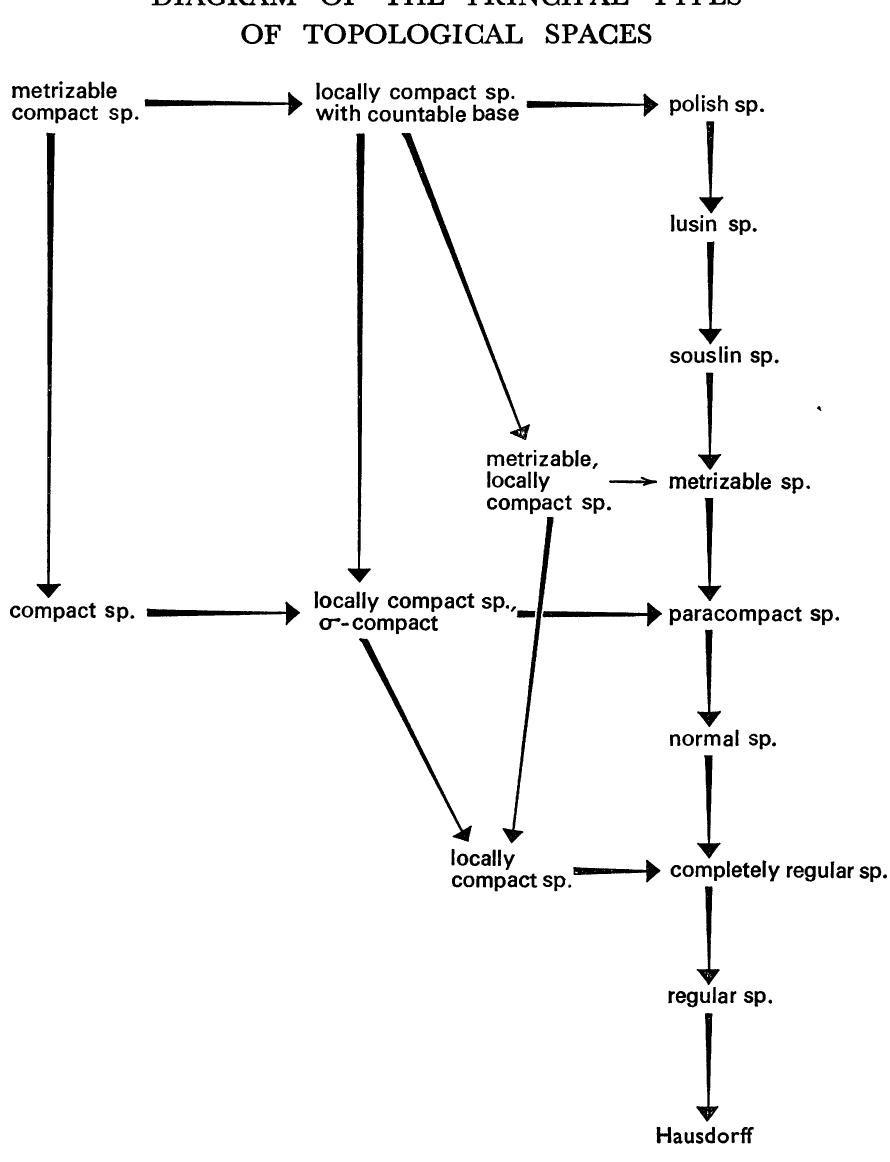
\includegraphics[keepaspectratio]{images/part002_2eb706e7.jpg}}

\section*{HISTORICAL NOTE}
\phantomsection
\addcontentsline{toc}{section}{Historical Note}

(Numbers in brackets refer to the bibliography at the end of this Note.)

As we remarked in the Historical Note to Chapter II, the notion of a metric space was introduced in 1906 by M. Fréchet, and developed some years later by F. Hausdorff in his ``Mengenlehre''. It acquired great importance after 1920, partly as a consequence of the fundamental work of S. Banach and his school on normed spaces and their applications to functional analysis, and also because of the significance of the notion of absolute value in the theory of numbers and algebraic geometry (where in particular the process of completion with respect to an absolute value has proved to be a powerful instrument).

The decade 1920-1930 saw a whole series of investigations into the properties of metric spaces. These studies, undertaken by the Moscow school, aimed especially at getting necessary and sufficient conditions for the metrizability of a given topology. This movement of ideas brought out the significance of the notion of a normal space, which had been defined by Tietze in 1923 but whose important role was recognized only as a consequence of the work of Urysohn {[}6{]} on the extension of continuous real-valued functions. Except for the trivial case of functions of a real variable, the problem of extending to the whole space a continuous real-valued function defined on a closed set was first considered (for the case of the plane) by H. Lebesgue {[}3{]}; before Urysohn's definitive result, it was solved for metric spaces by H. Tietze {[}4{]}. The generalization of this problem to include functions with values in an arbitrary topological space has acquired considerable importance in algebraic topology in the last few years. Recent work has also shown that in questions of this sort the notion of a normal space is not easily handled, since it allows too many possibilities of ``pathology''; it often has to be replaced by the more restrictive concept of paracompactness, introduced in 1944 by J. Dieudonné {[}9{]}. In this theory, the most remarkable result is the theorem of A. H. Stone {[}10{]} which states that every metrizable space is paracompact (*).

We have already noted (Historical Note to Chapter IV) the important work at the end of the nineteenth century and the beginning of the twentieth (E. Borel, Baire, Lebesgue, Osgood, W. H. Young) on the classification of point-sets in \(R^{n}\) , and on the classification and characterization of real-valued functions obtained from continuous functions by iterating the process of passing to the limit (with respect to sequences of functions). It was quickly realized that metric spaces, whose development after 1910 is largely the work of the Russian and Polish schools, formed a natural domain for investigations of this nature. Among other things, the study of metric spaces has shown clearly the fundamental role played in modern analysis by the notion of a meagre set and by the theorem on the countable intersection of dense open sets in a complete metric space ( \(§\ 5,\ no.\ 3,\ Theorem\ 1\) ), which was first proved (independently) by Osgood {[}1{]} for the real line and by Baire {[}2{]} for the spaces \(R^{n}\) .

On the other hand, Souslin in 1917 {[}5{]}, correcting an error of Lebesgue's, showed that the continuous image of a Borel set is not necessarily a Borel set; this led him to the definition and study of a larger class of sets, since called ``analytic sets'' or ``Souslin sets''. After Souslin's premature death this work was carried forward particularly by N. Lusin (whose ideas had inspired Souslin's work) and the Polish mathematicians (see {[}7{]} and {[}8{]}). The importance of these sets nowadays lies in their applications to the theory of integration (where, thanks to their special properties, they allow constructions which would be impossible for arbitrary measurable sets) and to modern potential theory, in which the fundamental theorem on the capacitability of Souslin sets, proved recently by G. Choquet {[}11{]}, has already shown itself to be rich in diverse applications.

\subsection*{BIBLIOGRAPHY}

{[}1{]} W. Osgood, Non-uniform convergence and the integration of series term by term, Amer. Journ. of Math., 19 (1897), pp.~155-190.

{[}2{]} R. BAIRE, Sur les fonctions de variables réelles, Ann. di Mat. (3), 3 (1899), p.~i.

{[}3{]} H. LEBESGUE, Sur le problème des Dirichlet, Rend. Circ. mat. di Palermo, 24 (1907), pp.~371-402.

{[}4{]} H. TIETZE, Über Funktionen, die auf einer abgeschlossenen Menge stetig sind, J. de Crelle, 145 (1915), pp.~9-14.

{[}5{]} M. SOUSLIN, Sur une définition des ensembles mesurables B sans nombres transfinis, C. R. Acad. Sci., 164 (1917), pp.~88-91.

{[}6{]} P. URYSOHN, Über die Mächtigkeit der zusammenhängenden Mengen, Math. Ann., 94 (1925), p.~262.

{[}7{]} N. Lusin, Leçons sur les ensembles analytiques et leurs applications, Paris (Gauthier-Villars), 1930.

{[}8{]} K. KURATOWSKI, Topologie I, 2nd edition, Warszawa-Vrocaw, 1948.

{[}9{]} J. DIEUDONNÉ, Une généralisation des espaces compacts, Journ. de Math. (9), 23 (1944), pp.~65-76.

{[}10{]} A. H. STONE, Paracompactness and product spaces, Bull. Amer. Math. Soc., 54 (1948), pp.~977-982.

{[}11{]} G. CHOQUET, Theory of capacities, Ann. Inst. Fourier, 5 (1953-1954) pp.~131-295.

\ResumeMainChapters
\chapter{Function spaces}

\section{\texorpdfstring{THE UNIFORMITY OF \(\mathfrak{S}\)-CONVERGENCE}{THE UNIFORMITY OF S-CONVERGENCE}}

Notation. If X and Y are any two sets, we recall that the set of all mappings of X into Y is denoted by \(\mathcal{F}(\mathbf{X};\mathbf{Y})\) , and may be identified with the product set \(\mathbf{Y}^{\mathbf{x}}\) (Set Theory, Chapter II, § 5, no. 2). For each subset H of \(\mathcal{F}(\mathbf{X};\mathbf{Y})\) and each \(x\in \mathbf{X}\) , we shall denote by \(\mathrm{H}(x)\) the set of elements \(u(x)\in \mathbf{Y}\) as \(u\) runs through H. If \(\Phi\) is a filter base on \(\mathcal{F}(\mathbf{X};\mathbf{Y})\) , we denote by \(\Phi (x)\) the filter base on Y formed by the sets \(\mathrm{H}(x)\) as H runs through \(\Phi\) . Finally, we recall that, for each \(u\in \mathcal{F}(\mathbf{X};\mathbf{Y})\) and each subset A of X, \(u|\mathrm{A}\) denotes the restriction of \(u\) to A, which is a mapping of A into Y; if H is a subset of \(\mathcal{F}(\mathbf{X};\mathbf{Y})\) , H\textbar A will denote the set of restrictions \(u|\mathrm{A}\) of functions \(u\in \mathrm{H}\) .

\subsection{THE UNIFORMITY OF UNIFORM CONVERGENCE}

Let X be a set and let Y be a uniform space. For each entourage V of Y, let \(W(V)\) denote the set of all pairs \((u, v)\) of mappings of X into Y such that \((u(x), v(x)) \in V\) for all \(x \in X\) . As V runs through the set of entourages of Y, the sets \(W(V)\) form a fundamental system of entourages of a uniformity on F(X; Y). For they clearly satisfy Axiom \((\mathrm{U}_{\mathrm{I}}^{\prime})\) (Chapter II, § 1, no. 1); if V, \(V'\) are two entourages of Y such that \(V \subset V'\) , we have \(W(V) \subset W(V')\) , and therefore the sets \(W(V)\) satisfy \((\mathrm{B}_{\mathrm{I}})\) (Chapter I, § 6, no. 3); we have \(\widehat{W(V)} = W(\overline{V}^{-1})\) so that \((\mathrm{U}_{\mathrm{II}}^{\prime})\) is satisfied; finally, the relations `` \((u(x), v(x)) \in V\) for all \(x \in X\)'' and `` \((v(x), w(x)) \in V\) for all \(x \in X\)'' imply the relation `` \((u(x), w(x)) \in V^{2}\) for all \(x \in X\)'' ; in other words, we have \(\widehat{W(V)} \subset W(\overline{V}^{2})\) , which proves \((\mathrm{U}_{\mathrm{III}}^{\prime})\) .

DEFINITION 1. The uniformity on the set \(\mathcal{F}(\mathbf{X};\mathbf{Y})\) which has as a fundamental system of entourages the set of subsets \(W(\mathbf{V})\) , where \(\mathbf{V}\) runs through the set of entourages of \(\mathbf{Y}\) , is called the uniformity of uniform convergence. The topology it induces is called the topology of uniform convergence. If a filter \(\Phi\) on \(\mathcal{F}(\mathbf{X};\mathbf{Y})\) converges to an element \(u_0\) with respect to this topology, \(\Phi\) is said to converge uniformly to \(u_0\) .

Note that the topology of uniform convergence on \(\mathcal{F}(\mathrm{X};\mathrm{Y})\) depends on the uniform structure of Y and not merely on the topology of Y (Exercise 4).

The uniform space obtained by endowing \(\mathcal{F}(\mathbf{X};\mathbf{Y})\) with the uniformity of uniform convergence is denoted by \(\mathcal{F}_u(\mathbf{X};\mathbf{Y})\) .

\subsection{\texorpdfstring{\(\mathfrak{S}\)-CONVERGENCE}{S-CONVERGENCE}}

DEFINITION 2. Let X be a set, Y a uniform space, S a set of subsets of X. The uniformity of uniform convergence in the sets of S, or simply the uniformity of S-convergence, is the coarsest uniformity on F(X; Y) which makes uniformly continuous the restriction mappings \(u \to u|A\) of F(X, Y) into the uniform spaces \(\mathcal{F}_u(A; Y)\) , where A runs through S. The uniform space obtained by endowing F(X; Y) with the uniformity of S-convergence is denoted by \(\mathcal{F}_{\mathfrak{S}}(X; Y)\) .

The topology induced by the uniformity of \(\mathfrak{S}\) -convergence is called the topology of \(\mathfrak{S}\) -convergence; it is the coarsest for which all the mappings \(u \to u|A\) of \(\mathcal{F}(X; Y)\) into \(\mathcal{F}_u(A; Y) (A \in \mathfrak{S})\) are continuous (Chapter II, § 2, no. 3, Proposition 4, Corollary).

A filter \(\Phi\) on \(\mathcal{F}(\mathbf{X};\mathbf{Y})\) converges to \(u_{0}\) with respect to the topology of \(\mathfrak{S}\) -convergence if and only if \(u|\mathrm{A}\) converges uniformly to \(u_{0}|\mathrm{A}\) with respect to \(\Phi\) for all \(\mathrm{A}\in \mathfrak{S}\) (Chapter I, § 7, no. 6, Proposition 10), and \(\Phi\) is therefore said to converge uniformly to \(u_{0}\) on the sets of \(\mathfrak{S}\) .

A filter base \(\Phi\) on \(\mathcal{F}_{\mathfrak{S}}(\mathbf{X};\mathbf{Y})\) is a Cauchy filter base if and only if, for each \(\mathbf{A}\in\mathfrak{S}\) , the image of \(\Phi\) under the mapping \(u\to u|\mathbf{A}\) is a Cauchy filter base on \(\mathcal{F}_{u}(\mathbf{A};\mathbf{Y})\) (Chapter II, § 3, no. 1, Proposition 4).

Let \(f\) be a mapping of a topological (resp. uniform) space \(Z\) into \(\mathcal{F}_{\mathfrak{S}}(X; Y)\) . Then \(f\) is continuous (resp. uniformly continuous) if and only if, for each \(A \in \mathfrak{S}\) , the mapping \(z \to f(z)|A\) of \(Z\) into \(\mathcal{F}_u(A; Y)\) is continuous (resp. uniformly continuous) (Chapter I, § 2, no. 3, Proposition 4; Chapter II, § 2, no. 3, Proposition 4).

Finally, let \(\mathbf{M}\) be a subset of \(\mathcal{F}_{\mathfrak{S}}(\mathbf{X};\mathbf{Y})\) ; then \(\mathbf{M}\) is precompact if and only if, for each \(\mathbf{A} \in \mathfrak{S}\) , the set of restrictions \(u|\mathbf{A}\) for \(u \in \mathbf{M}\) is a precompact subset of \(\mathcal{F}_u(\mathbf{A};\mathbf{Y})\) (Chapter II, § 4, no. 2, Proposition 3).

Remarks. 1) The general definition of the entourages of an initial uniformity (Chapter II, § 2, no. 3, Proposition 4) shows that a fundamental system of entourages of \(\mathcal{F}_{\mathfrak{S}}(\mathrm{X};\mathrm{Y})\) may be obtained as follows: for each \(\mathbf{A}\in \mathfrak{S}\) and each entourage \(\mathbf{V}\) of a fundamental system of entourages \(\mathfrak{B}\) of \(\mathbf{Y}\) , let \(W(\mathbf{A},\mathbf{V})\) be the set of all pairs of mappings \((u,v)\) of \(\mathbf{X}\) into \(\mathbf{Y}\) such that \((u(x),v(x))\in \mathbf{V}\) for each \(x\in \mathbf{A}\) ; as \(\mathbf{A}\) runs through \(\mathfrak{S}\) and \(\mathbf{V}\) runs through \(\mathfrak{B}\) , the finite intersections of the sets \(W(\mathbf{A},\mathbf{V})\) form a fundamental system of entourages of \(\mathcal{F}_{\mathfrak{S}}(\mathrm{X};\mathrm{Y})\) .

This description shows immediately that if \(\mathfrak{S},\mathfrak{S}'\) are two sets of subsets of \(\mathbf{X}\) such that \(\mathfrak{S} \subset \mathfrak{S}'\) , then the uniformity of \(\mathfrak{S}'\) -convergence is finer than that of \(\mathfrak{S}\) -convergence.

\begin{enumerate}
\def\labelenumi{\arabic{enumi})}
\setcounter{enumi}{1}
\tightlist
\item
  However, the uniformity of \(\mathfrak{S}\) -convergence is unaltered by replacing \(\mathfrak{S}\) by the set \(\mathfrak{S}'\) of all subsets of X which are contained in finite unions of sets of \(\mathfrak{S}\) . In the study of \(\mathfrak{S}\) -convergence we may therefore always restrict ourselves to the case where the set \(\mathfrak{S}\) satisfies the following two conditions:
\end{enumerate}

\((\mathbf{F}_{\mathbf{I}}^{\prime})\) Every subset of a set of \(\mathfrak{S}\) belongs to \(\mathfrak{S}\) .

\((F_{\mathrm{II}}^{\prime})\) Every finite union of sets of \(\mathfrak{S}\) belongs to \(\mathfrak{S}\) .

If \((\mathbf{F}_{\mathrm{II}}^{\prime})\) is satisfied, we obtain a fundamental system of entourages of \(\mathcal{F}_{\mathfrak{S}}(\mathbf{X};\mathbf{Y})\) by taking all the sets \(\boldsymbol{W}(\mathrm{A},\mathrm{V})\) , where A runs through S and V runs through a fundamental system of entourages of Y.

\begin{enumerate}
\def\labelenumi{\arabic{enumi})}
\setcounter{enumi}{2}
\tightlist
\item
  The uniformity of \(\mathfrak{S}\) -convergence is the inverse image, under the mapping \(u \to (u|\mathbf{A})_{\mathbf{A} \in \mathfrak{S}}\) of \(\mathcal{F}(\mathbf{X}; \mathbf{Y})\) into \(\prod_{\mathbf{A} \in \mathfrak{S}} \mathcal{F}_u(\mathbf{A}; \mathbf{Y})\) , of the uniformity of this product space (Chapter II, § 2, no. 6, Proposition 8). If \(\mathfrak{S}\) is a covering of \(\mathbf{X}\) , this mapping is injective and \(\mathcal{F}_{\mathfrak{S}}(\mathbf{X}; \mathbf{Y})\) is therefore isomorphic to the uniform subspace of \(\prod_{\mathbf{A} \in \mathfrak{S}} \mathcal{F}_u(\mathbf{A}; \mathbf{Y})\) which is the image of this mapping.
\end{enumerate}

PROPOSITION 1. If Y is Hausdorff and S is a covering of X, then the space \(\mathcal{F}_{\mathfrak{S}}(X;Y)\) is Hausdorff.

Let \(u, v\) be two elements of \(\mathcal{F}_{\mathfrak{S}}(\mathrm{X}; \mathrm{Y})\) such that \((u, v) \in W(\mathrm{A}, \mathrm{V})\) for every entourage \(\mathrm{V}\) of \(\mathrm{Y}\) and every \(\mathrm{A} \in \mathfrak{S}\) . Since \(\mathrm{Y}\) is Hausdorff it follows that \(u\) and \(v\) coincide on every set \(\mathrm{A} \in \mathfrak{S}\) , and since \(\mathfrak{S}\) covers \(\mathrm{X}\) we must have \(u = v\) .

Remarks. 4) Let H be a subset of \(\mathcal{F}(\mathbf{X};\mathbf{Y})\) . By abuse of language, the uniformity (resp. topology) induced on H by the uniformity (resp. topology) of \(\mathfrak{S}\) -convergence on \(\mathcal{F}(\mathbf{X};\mathbf{Y})\) is called the uniformity (resp. topology) of \(\mathfrak{S}\) -convergence on the set H.

\begin{enumerate}
\def\labelenumi{\arabic{enumi})}
\setcounter{enumi}{4}
\tightlist
\item
  Let L be a set filtered by a filter \(\mathfrak{G}\) , and let \(\lambda \to u_{\lambda}\) be a mapping of L into \(\mathcal{F}_{\mathfrak{S}}(\mathbf{X};\mathbf{Y})\) which has a limit \(v\) with respect to \(\mathfrak{G}\) ; we say then that, with respect to the filter \(\mathfrak{G}\) , the mappings \(u_{\lambda}\) of X into Y converge uniformly to \(v\) {[}or that the family \((u_{\lambda})\) is uniformly convergent to \(v\) {]} in every set of \(\mathfrak{S}\) . If \(\mathbf{L} = \mathbf{N}\) and \(\mathfrak{G}\) is the Fréchet filter, we omit mention of \(\mathfrak{G}\) in this statement.
\end{enumerate}

More particularly, suppose that there is a commutative and associative law of composition (written additively) defined on Y. If \((u_{n})\) is any sequence of mappings of X into Y, let \(v_{n}\) be the mapping defined by

\[
v _ {n} (x) = \sum_ {k = 0} ^ {n} u _ {k} (x) \quad (n \in \mathbf {N});
\]

we say that the series whose general term is \(u_n\) is uniformly convergent in every set of \(\mathfrak{S}\) if the sequence \((v_n)\) is uniformly convergent in every set of \(\mathfrak{S}\) . Likewise we define a uniformly summable family \((u_\lambda)_{\lambda \in \mathbf{L}}\) of mappings of \(\mathbf{X}\) into \(\mathbf{Y}\) by considering the mappings \(x \to \sum_{\lambda \in \mathbf{J}} u_\lambda(x)\) for all finite subsets

J of L and the limit of these mappings in \(\mathcal{F}_{\mathfrak{S}}(\mathbf{X};\mathbf{Y})\) with respect to the directed set of finite subsets of L (Chapter III, § 5, no. 1).

\begin{enumerate}
\def\labelenumi{\arabic{enumi})}
\setcounter{enumi}{5}
\tightlist
\item
  It follows immediately from Definitions 1 and 2 that, for every \(x \in \bigcup_{\mathbf{A} \in \mathfrak{S}} \mathbf{A}\) , the mapping \(u \to v(x)\) of \(\mathcal{F}_{\mathfrak{S}}(\mathbf{X}; \mathbf{Y})\) into Y is uniformly continuous. Hence, in particular, if \(\overline{\mathbf{H}}\) denotes the closure of a subset H of \(\mathcal{F}_{\mathfrak{S}}(\mathbf{X}; \mathbf{Y})\) , we have \(\overline{\mathbf{H}}(x) \subset \overline{\mathbf{H}(x)}\) for all \(x \in \bigcup_{\mathbf{A} \in \mathfrak{S}} \mathbf{A}\) (Chapter I, § 2, no. 1, Theorem 1).
\end{enumerate}

\subsection{\texorpdfstring{EXAMPLES OF \(\mathfrak{S}\)-CONVERGENCE}{EXAMPLES OF S-CONVERGENCE}}

I. Uniform convergence in a subset of X. Let A be a subset of X and take \(\mathfrak{S} = \{\mathrm{A}\}\) . The uniformity (resp. topology) of \(\mathfrak{S}\) -convergence is then called the uniformity (resp. topology) of uniform convergence in A; if a filter \(\Phi\) on \(\mathcal{F}_{\mathfrak{S}}(\mathrm{X};\mathrm{Y})\) converges to \(u_0\) , it is said to converge to \(u_0\) uniformly in A. When \(\mathrm{A} = \mathrm{X}\) we recover the structure of uniform convergence defined in no. 1.

\begin{enumerate}
\def\labelenumi{\Roman{enumi}.}
\setcounter{enumi}{1}
\tightlist
\item
  Pointwise convergence in a subset of X. Let A be a subset of X, and take S to be the set of all subsets of X which consist of a single point belonging to A (by Remark 2 of no. 2 it comes to the same thing if we take S to be the set of all finite subsets of A). The uniformity (resp. topology) of S-convergence is then called the uniformity (resp. topology) of pointwise convergence in A; if a filter Φ on \(\mathcal{F}_{\mathfrak{S}}(\mathbf{X};\mathbf{Y})\) converges to \(u_0\) , it is said to converge to \(u_0\) pointwise in A. This will be the case if and only if, for each \(x\in \mathbf{A}\) , \(u_0(x)\) is a limit of \(u(x)\) with respect to the filter Φ.
\end{enumerate}

In particular, when A = X, the uniformity (resp. topology) of pointwise convergence in X is called simply the uniformity (resp. topology) of pointwise convergence; the uniform space obtained by endowing \(\mathcal{F}(X; Y)\) with this structure is denoted by \(\mathcal{F}_{s}(X; Y)\) . Note that the topology of pointwise convergence is just the product topology on \(Y^{X}\) and therefore depends only on the topology of Y, and not on its uniform structure.

\begin{enumerate}
\def\labelenumi{\Roman{enumi}.}
\setcounter{enumi}{2}
\tightlist
\item
  Compact convergence. Suppose that X is a topological space, and take S to be the set of all compact subsets of X. The uniformity (resp. the topology) of S-convergence is then called the uniformity (resp. the topology) of compact convergence, and the uniform space obtained by endowing \(\mathcal{F}(X;Y)\) with this uniformity is denoted by \(\mathcal{F}_{c}(X;Y)\) . The structure of compact convergence is coarser than that of uniform convergence, and the two coincide if X is compact; also it is finer than the structure of pointwise convergence, and these two coincide if X is discrete.
\end{enumerate}

If X is a uniform space we can define on \(\mathcal{F}(X;Y)\) the uniformity of precompact convergence by taking S to be the set of all precompact subsets of X. Again, if X is a metric space we may take S to be the set of all bounded subsets of X; the uniformity of S-convergence is then called the uniformity of bounded convergence.

\subsection{\texorpdfstring{PROPERTIES OF THE SPACES \(\mathcal{F}_{\mathfrak{G}}(\mathbf{X};\mathbf{Y})\)}{PROPERTIES OF THE SPACES F SUB G (X;Y)}}

PROPOSITION 2. Let \(\mathbf{X}_1, \mathbf{X}_2\) be two sets, let \(\mathbf{Y}\) be a uniform space and let \(\mathfrak{S}_i\) be a set of subsets of \(\mathbf{X}_i\) ( \(i = 1, 2\) ) and \(\mathfrak{S}_1 \times \mathfrak{S}_2\) the set of subsets of \(\mathbf{X}_1 \times \mathbf{X}_2\) of the form \(\mathbf{A}_1 \times \mathbf{A}_2\) , where \(\mathbf{A}_i \in \mathfrak{S}_i\) , \(i = 1, 2\) . Then the canonical bijection

\[
\mathscr {F} \left(\mathrm{X} _ {1} \times \mathrm{X} _ {2}; \mathrm{Y}\right)\rightarrow \mathscr {F} \left(\mathrm{X} _ {1}; \mathscr {F} \left(\mathrm{X} _ {2}; \mathrm{Y}\right)\right)
\]

(Set Theory, R, § 4, no. 14) is an isomorphism of the uniform space

\[
\mathcal {F} _ {\mathfrak {S} _ {1} \times \mathfrak {S} _ {2}} (\mathrm{X} _ {1} \times \mathrm{X} _ {2}; \mathrm{Y})
\]

onto \(\mathcal{F}_{\mathfrak{S}_1}(\mathbf{X}_1;\mathcal{F}_{\mathfrak{S}_2}(\mathbf{X}_2;\mathbf{Y}))\)

Let \(\mathbf{V}\) be an entourage of \(\mathbf{Y}\) and let \(\mathbf{A}_i\in \mathfrak{S}_i\) ( \(i = 1,2\) ); then it follows immediately from the definitions that \(W(\mathbf{A}_1\times \mathbf{A}_2,\mathbf{V})\) is identified with \(W(\mathbf{A}_1,W(\mathbf{A}_2,\mathbf{V}))\) by the canonical bijection, and the result is immediate.

PROPOSITION 3. a) Let X be a set; let S be a set of subsets of X; let Y, Y' be two uniform spaces; and let f: Y → Y' be a uniformly continuous mapping. Then the mapping u → f ∘ u of F\_S(X; Y) into F\_S(X; Y') is uniformly continuous.

\begin{enumerate}
\def\labelenumi{\alph{enumi})}
\setcounter{enumi}{1}
\tightlist
\item
  Let \(\mathbf{X}, \mathbf{X}'\) be two sets; let \(\mathfrak{S}\) (resp. \(\mathfrak{S}'\) ) be a set of subsets of \(\mathbf{X}\) (resp. \(\mathbf{X}'\) ); let \(\mathbf{Y}\) be a uniform space; and let \(g: \mathbf{X}' \to \mathbf{X}\) be a mapping such that, for each \(\mathbf{A}' \in \mathfrak{S}'\) , \(g(\mathbf{A}')\) is contained in a finite union of sets of \(\mathfrak{S}\) . Then the mapping \(u \to u \circ g\) of \(\mathcal{F}_{\mathfrak{S}}(\mathbf{X}, \mathbf{Y})\) into \(\mathcal{F}_{\mathfrak{S}'}(\mathbf{X}', \mathbf{Y})\) is uniformly continuous.
\end{enumerate}

PROPOSITION 4. Let X, Y be two sets, let \((\mathbf{X}_{\lambda})_{\lambda \in \mathbf{L}}\) be a family of sets and let \((\mathrm{Y}_{\mu})_{\mu \in \mathbf{M}}\) be a family of uniform spaces. For each \(\lambda \in \mathbf{L}\) , let \(\mathfrak{S}_{\lambda}\) be a set of subsets of \(\mathbf{X}_{\lambda}\) , let \(g_{\lambda}\) be a mapping of \(\mathbf{X}_{\lambda}\) into X, and let \(\mathfrak{S}\) be the set of subsets of X which is the union of the sets \(g_{\lambda}(\mathfrak{S}_{\lambda})\) . For each \(\mu \in \mathbf{M}\) , let \(f_{\mu}\) be a mapping of Y into \(Y_{\mu}\) , and endow Y with the coarsest uniformity for which the \(f_{\mu}\) are uniformly continuous. Then the uniformity of S-convergence on \(\mathcal{F}(X;Y)\) is the coarsest uniformity which makes uniformly continuous the mappings \(u \to f_{\mu} \circ u \circ g_{\lambda}\) of \(\mathcal{F}(X;Y)\) into \(\mathcal{F}_{\mathfrak{S}_{\lambda}}(X_{\lambda},Y_{\mu})\) .

These propositions are immediate consequences of the description of a fundamental system of entourages for the uniformity of S-convergence given in no. 2, Remark 1; the details of the proofs are left to the reader. Proposition 4 implies, in particular:

COROLLARY. Let X be a set, let \((\mathrm{Y}_{t})_{t\in\mathbf{I}}\) be a family of uniform spaces and let S be a set of subsets of X. If we endow \(\prod_{t\in I}Y_{t}\) with the product uniformity, the canonical bijection of the uniform space \(\mathcal{F}_{\mathfrak{S}}\left(\mathrm{X},\prod_{t\in\mathbf{I}}\mathrm{Y}_{t}\right)\) onto the product uniform space \(\prod_{t\in\mathbf{I}}\mathcal{F}_{\mathfrak{S}}(\mathrm{X};\mathrm{Y}_{t})\) (Set Theory, R, § 4, no. 13) is an isomorphism.

\subsection{\texorpdfstring{COMPLETE SUBSETS OF \(\mathcal{F}_{\mathfrak{S}}(\mathbf{X};\mathbf{Y})\)}{COMPLETE SUBSETS OF F SUB S (X;Y)}}

PROPOSITION 5. Let \(\Phi\) be a set, Y a uniform space and \(\mathfrak{S}\) a set of subsets of X. Then a filter \(\Phi\) on \(\mathcal{F}_{\mathfrak{S}}(\mathbf{X};\mathbf{Y})\) converges to \(u_0\) if and only if \(\Phi\) is a Cauchy filter with respect to the uniformity of \(\mathfrak{S}\) -convergence and converges pointwise to \(u_0\) in \(\mathbf{B} = \bigcup_{\mathbf{A}\in \mathfrak{S}}\mathbf{A}\) .

Since the structure of pointwise convergence in B is coarser than that of S-convergence, it is enough to show that for each \(A \in S\) and each closed entourage V of Y, \(W(A, V)\) is closed in B with respect to the topology of pointwise convergence (Chapter II, § 3, no. 3, Proposition 7). Now \(W(A, V)\) is the intersection of the inverse images of V under the mappings \((u, v) \to (u(x), v(x))\) as x runs through A; these mappings are continuous with respect to the topology of pointwise convergence (no. 2, Remark 6), and the result follows.

COROLLARY 1. A subspace H of \(\mathcal{F}_{\mathfrak{S}}(\mathbf{X};\mathbf{Y})\) is complete if and only if, for each Cauchy filter \(\Phi\) on H, there exists \(u_0\in \mathbf{H}\) such that \(\Phi\) converges pointwise to \(u_0\) in \(\mathbf{B} = \bigcup_{\mathbf{A}\in \mathfrak{S}}\mathbf{A}\) .

This follows immediately from Proposition 5.

COROLLARY 2. Let \(\mathfrak{S}_1, \mathfrak{S}_2\) be two sets of subsets of X, whose union is the same and which are such that \(\mathfrak{S}_1 \subset \mathfrak{S}_2\) , and let H be a subset of \(\mathcal{F}(X; Y)\) . Then if H is complete with respect to \(\mathfrak{S}_1\) -convergence, it is complete with respect to \(\mathfrak{S}_2\) -convergence.

For every Cauchy filter with respect to \(S_{2}\) -convergence is also a Cauchy filter with respect to \(S_{1}\) -convergence, and we may apply Corollary 1.

COROLLARY 3. Let H be a subset of \(\mathcal{F}(\mathbf{X};\mathbf{Y})\) such that, for each

\[
x \notin \mathrm{B} = \bigcup_ {\mathrm{A} \in \mathfrak {S}} \mathrm{A},
\]

the closure of \(\mathbf{H}(x)\) in \(\mathbf{Y}\) is a complete subspace of \(\mathbf{Y}\) . Then the closure \(\overline{\mathbf{H}}\) of \(\mathbf{H}\) in \(\mathcal{F}_{\mathfrak{S}}(\mathbf{X};\mathbf{Y})\) is a complete subspace.

Let \(\Phi\) be a Cauchy filter on \(\overline{\mathbf{H}}\) , and define a mapping \(v: \mathbf{X} \to \mathbf{Y}\) as follows. If \(x \in \mathbf{B}\) , \(\Phi(x)\) is a Cauchy filter on \(\overline{\mathbf{H}(x)}\) (no. 2, Remark 6), hence by hypothesis it has at least one limit point; take \(v(x)\) to be one of these limits. If \(x \notin \mathbf{B}\) , take \(v(x)\) to be any point of \(\mathbf{Y}\) . With this definition of \(v\) , it is clear that \(\Phi\) converges pointwise to \(v\) in \(\mathbf{B}\) , and \(v\) is therefore a limit of \(\Phi\) in \(\mathcal{F}_{\mathfrak{S}}(\mathbf{X}; \mathbf{Y})\) by Proposition 5.

In particular, if Y is complete, the hypothesis of Corollary 3 of Proposition 5 is satisfied for every \(H \subset \mathcal{F}(X; Y)\) ; hence:

THEOREM 1. Let X be a set, let S be a set of subsets of X, and let Y be a complete uniform space. Then the uniform space \(\mathcal{F}_{\mathfrak{S}}(X;Y)\) is complete.
